% =================================================================================================
% File:			client_tier/controller.tex
% Description:	Defiinisce la sezione relativa al front-end dell'applicazione
% Created:		2015-04-07
% Author:		Tesser Paolo
% Email:		tesser.paolo@mashup-unipd.it
% =================================================================================================
% Modification History:
% Version		Modifier Date		Change											Author
% 0.0.1 		2015-04-07 			creato scheletro								Tesser Paolo
% =================================================================================================
% 0.0.2			2015-04-07			scheletro delle classi dei pack					Tesser Paolo
% ================================================================================================
% 0.0.3			2015-04-08			descrizioni classi del pack controller_public	Tesser Paolo
% ================================================================================================
% 0.0.4			2015-04-08			inserite relazioni tra le classi				Tesser Paolo
% ================================================================================================
% 0.0.5			2015-04-09			completata descrizione classi					Tesser Paolo
% ================================================================================================
%

% CONTENUTO DEL CAPITOLO

\subsubsection{client::controller} % (fold)
\label{ssub:bdsm_app_client_controller}
Le classi definite per la gestione dell'indirizzamento delle pagine HTML dell'applicazione, e cioè quelle terminanti con \textbf{Route}, rappresentano delle configurazioni. Questo implica che non possiedono metodi o attributi, ma al massimo utilizzano servizi per attuare il loro compito che vengono descritti nella nota introduttiva in \ref{sub:client}. La zona quindi dedicata a quei valori sarà marcata come specificato in \ref{sub:note_specifica} e non verrà fornita nessuna immagine.


\begin{figure}[htbp]
	\centering
	\centerline{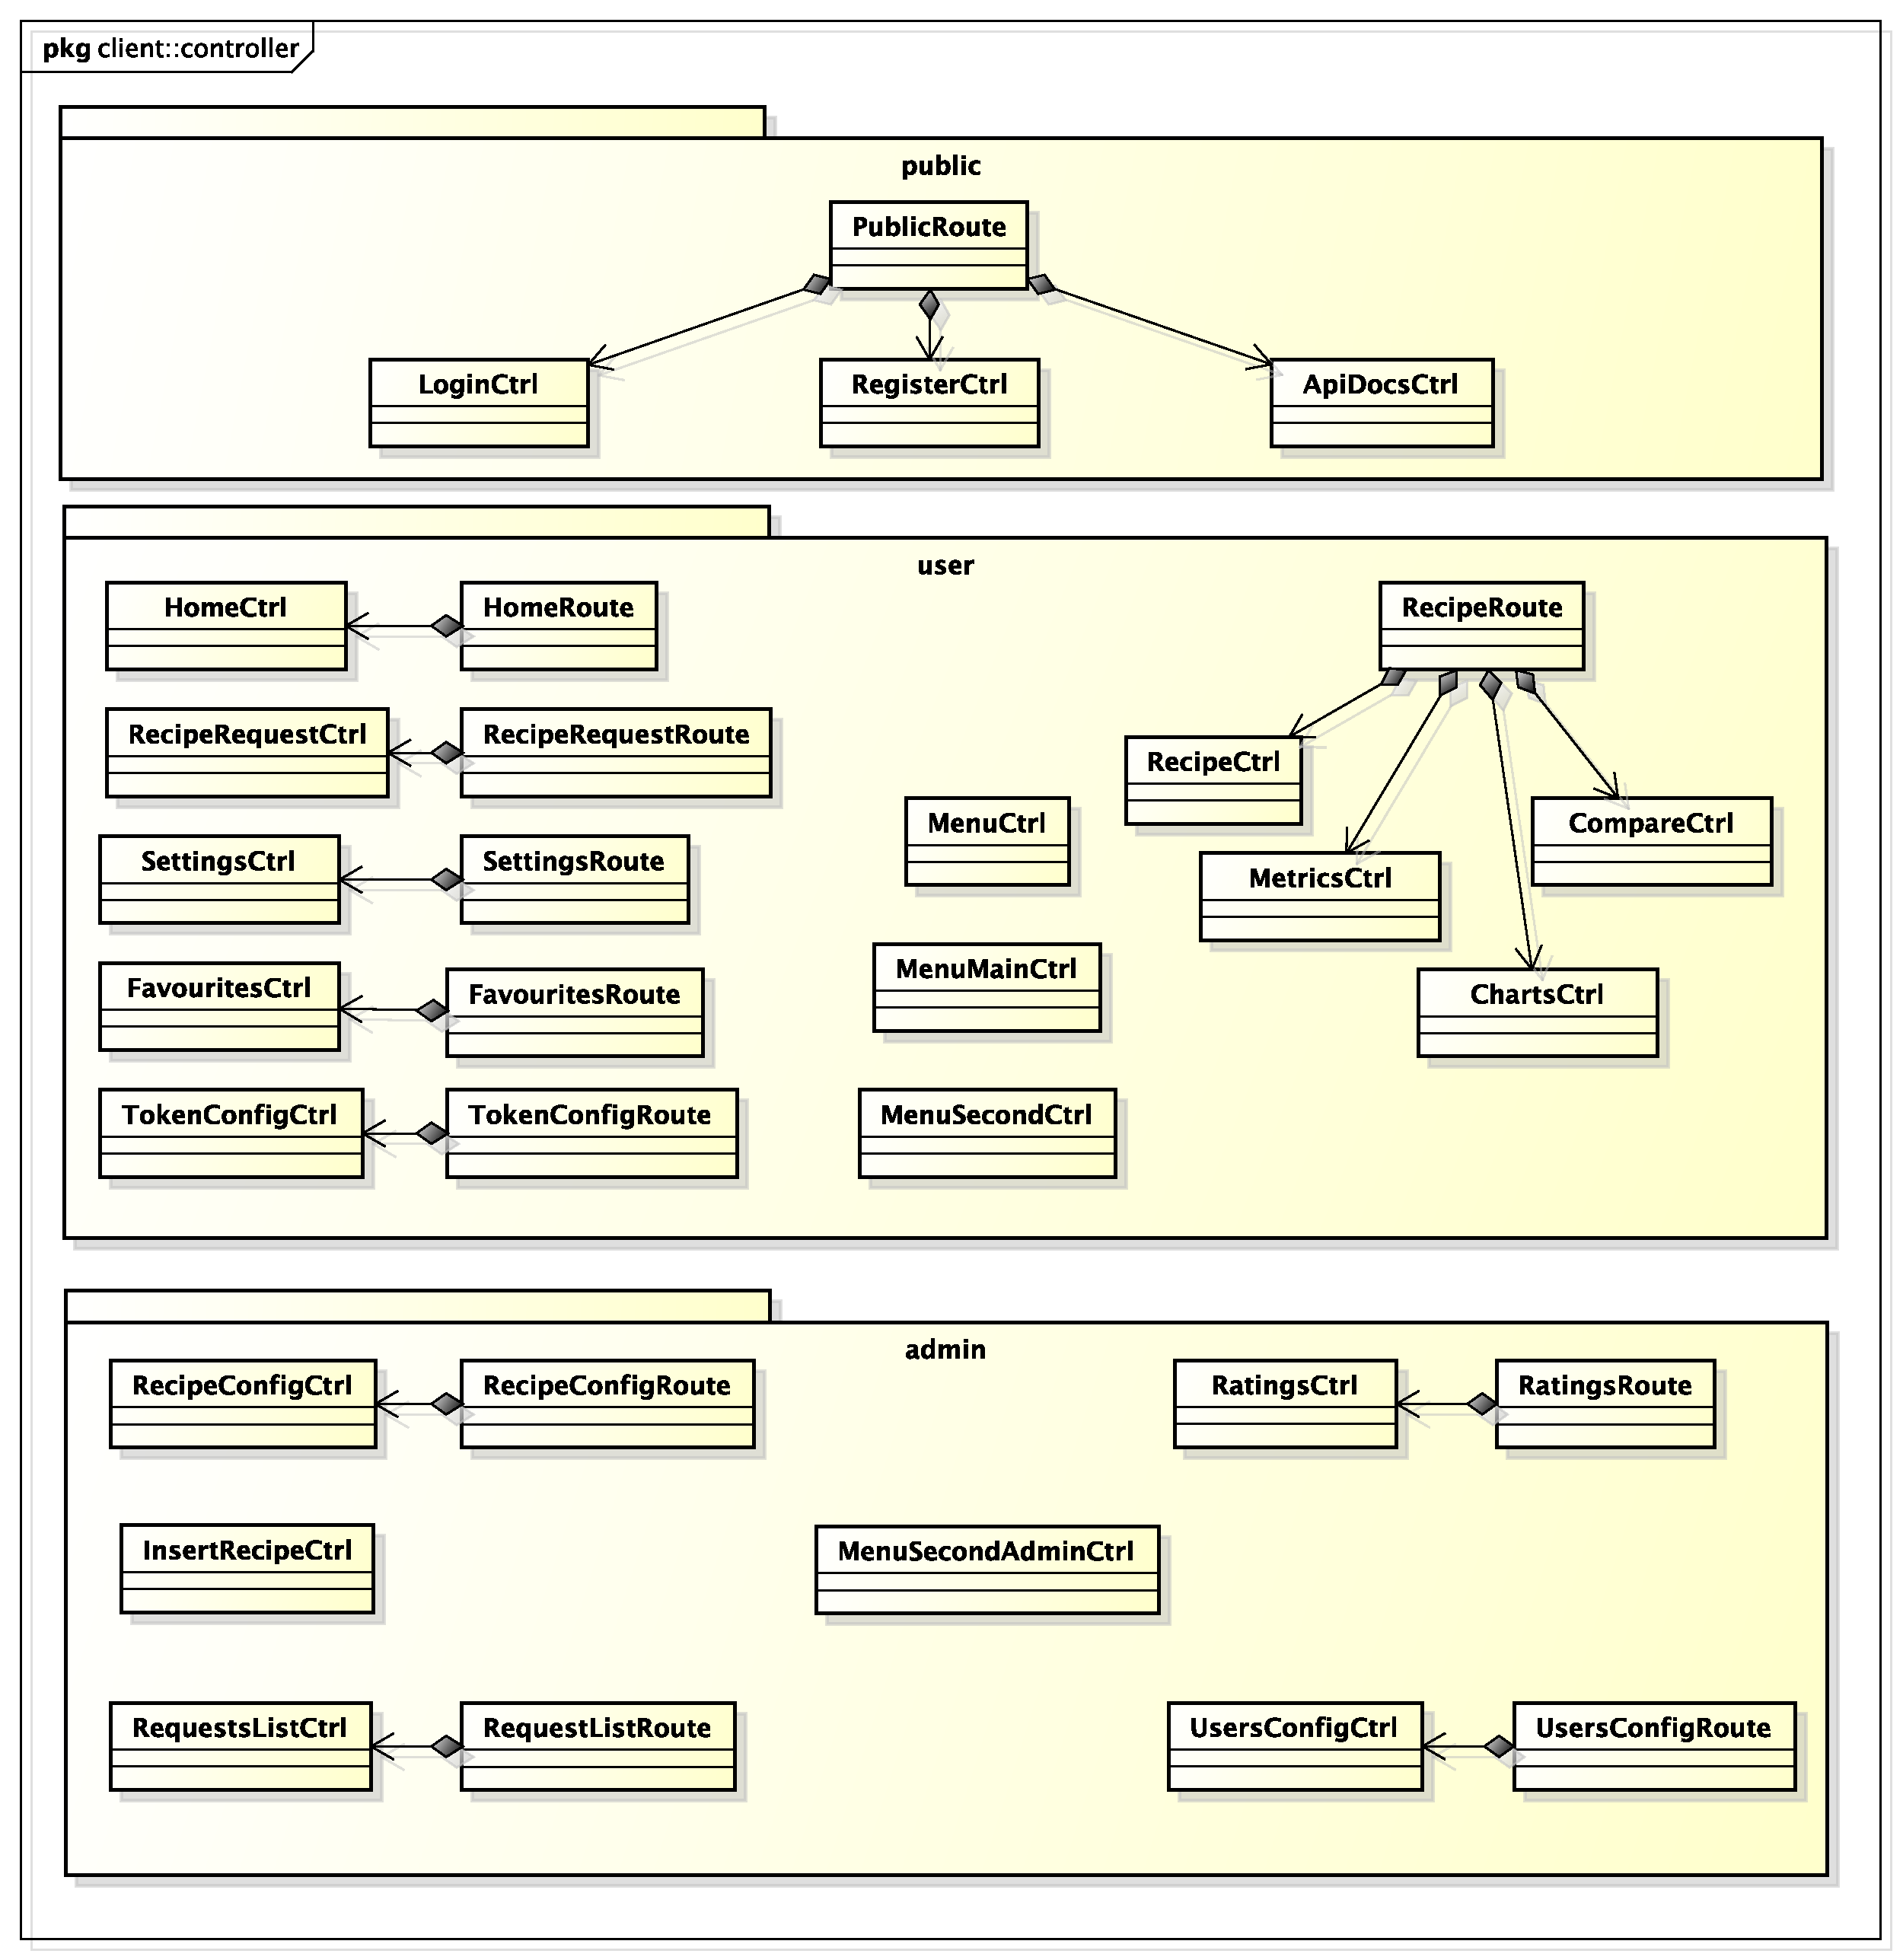
\includegraphics[scale=0.4]{./images/client/client_controller.pdf}}
	\caption{Package - client::controller}
\end{figure}

\begin{itemize}
	\item \textbf{Descrizione}: è il package che contiene le componenti che contengono i controller dell'applicazione e che incapsulano le funzionalità di two-way data binding tra le View e il Model. In esse è contenuta la logica applicativa riguardante le diverse pagine HTML;
	\item \textbf{Padre}: client;
	\item \textbf{Package contenuti}:
		\begin{itemize}
			\item client::controller::public
			\item client::controller::user
			\item client::controller::admin
		\end{itemize}
	\item \textbf{Interazione con altri componenti}:
		\begin{itemize}
			\item client::model
			\item client::view
		\end{itemize}
\end{itemize}
% subsubsection bdsm_app_client_controller (end)


\subsubsection{client::controller::public} % (fold)
\label{ssub:bdsm_app_client_controller_public}
\begin{figure}[htbp]
	\centering
	\centerline{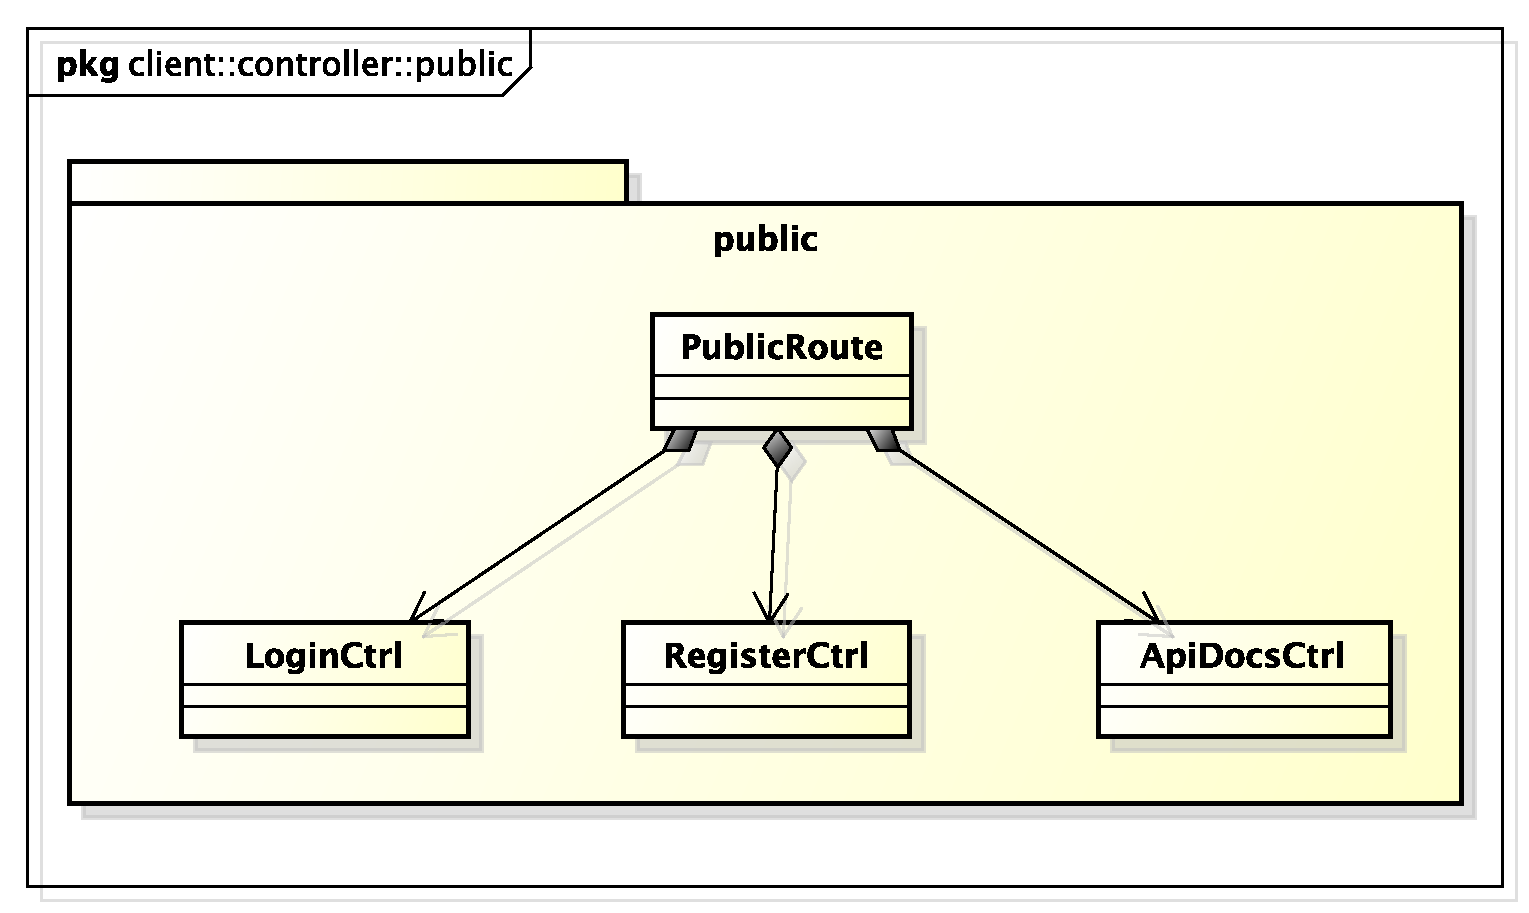
\includegraphics[scale=0.6]{./images/client/client_controller_public.pdf}}
	\caption{Package - client::controller::public}
\end{figure}

\begin{itemize}
	\item \textbf{Descrizione}: è il package che contiene le classi che controllano le decisioni di che pagine HTML mostrare all'utente che non si è ancora autenticato e di quali operazioni poter effettuare su di esse;
	\item \textbf{Padre}: client::controller
	\item \textbf{Interazione con altri componenti}:
		\begin{itemize}
			\item client::model::public
			\item client::view::public
		\end{itemize}
\end{itemize}

	\paragraph{Classi} % (fold)
		\subparagraph{client::controller::public::PublicRoute} % (fold)
		\label{subp:bdsm_app_client_controller_public_publicrouteconfig}

		\begin{itemize}
			\item \textbf{Descrizione}: la classe serve a gestire l'indirizzamento e l'assegnazione di uno stato al template HTML riguardante le pagine che può visualizzare un utente non autenticato, quali quella di autenticazione, di registrazione o di visione della documentazione dei servizi REST offerti;
			\item \textbf{Utilizzo}: viene utilizzata per reindirizzare l'utente al template HTML adeguato in caso si voglia o autenticare o registrare al sistema, o visualizzare i servizi REST offerti, ed assegnare al template scelto il controller opportuno per gestire i diversi compiti. Nel caso l'utente fosse già autenticato, la classe provvederà a reindirizzarlo all'URL associato alla Home;
			\item \textbf{Relazioni con altre classi}:
				\begin{itemize}
					\item client::view::public::Login
					\item client::view::public::Register
					\item client::view::public::ApiDocs
					\item client::controller::public::LoginCtrl
					\item client::controller::public::RegisterCtrl
					\item client::controller::public::ApiDocsCtrl
				\end{itemize}
				\item \textbf{Attributi associati allo \$scope}: N/A
				\item \textbf{Metodi associati allo \$scope e privati}: N/A
				\item \textbf{Servizi AngularJS utilizzati}:
					\begin{itemize}
						\item \$stateProvider
					\end{itemize}
		\end{itemize}
		% subparagraph bdsm_app_client_controller_public_publicrouteconfig (end)

		\subparagraph{client::controller::public::LoginCtrl} % (fold)
		\label{subp:bdsm_app_client_controller_public_loginctrl}
			\begin{figure}[htbp]
				\centering
				\centerline{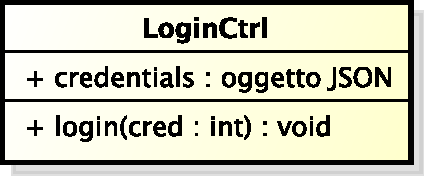
\includegraphics[scale=0.7]{./images/client/classes/controller/login_ctrl.pdf}}
				\caption{Classe - client::controller::public::LoginCtrl}
			\end{figure}
			\begin{itemize}
				\item \textbf{Descrizione}: la classe è il controller che serve a gestire la logica applicativa riguardante l'autenticazione al sistema;
				\item \textbf{Utilizzo}: viene utilizzata per gestire le operazioni di autenticazione al sistema qualora un utente non autenticato decidesse di effettuare l'accesso. Richiamando quindi i servizi che mettono in comunicazione il client con il server, verifica le credenziali ed effettua un reindirizzamento alla Home qualora fossero valide;
				\item \textbf{Relazioni con altre classi}:
					\begin{itemize}
						\item client::model::services::AuthService
						\item client::view::public::Login
						\item client::controller::public::PublicRoute
					\end{itemize}

				\item \textbf{Attributi associati allo \$scope}:
					\begin{itemize}

						\item \textcolor{forestgreen}{\texttt{+ credentials : oggetto JSON}}
							\begin{description}
								\item \textbf{Descrizione}: oggetto nel formato JSON che contiene il valore iniziale dei campi mail e password che inizialmente saranno vuoti. Il formato dell'oggetto JSON è il seguente:
								\begin{verbatim}
									{
									    email: 'info@mashup-unipd.it',
									    pwd: 'password'
									}
								\end{verbatim}
							\end{description}

					\end{itemize}

				\item \textbf{Metodi associati allo \$scope e privati}:
					\begin{itemize}
						\item \textcolor{forestgreen}{\texttt{+ login(cred)}}
							\begin{description}
								\item \textbf{Descrizione}: gli vengono passati i dati dalla view e viene invocato il metodo login della classe AuthService.
							\end{description}

					\end{itemize}

				\item \textbf{Servizi AngularJS utilizzati}: N/A

			\end{itemize}
		% subparagraph bdsm_app_client_controller_public_loginctrl (end)

		\subparagraph{client::controller::public::RegisterCtrl} % (fold)
		\label{subp:bdsm_app_client_controller_public_registerctrl}
			\begin{figure}[htbp]
				\centering
				\centerline{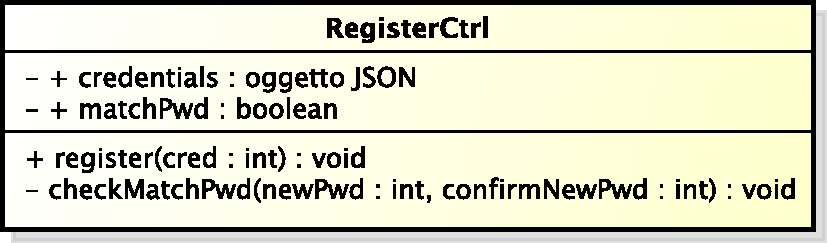
\includegraphics[scale=0.7]{./images/client/classes/controller/register_ctrl.pdf}}
				\caption{Classe - client::controller::public::RegisterCtrl}
			\end{figure}
			\begin{itemize}
				\item \textbf{Descrizione}: la classe è il controller che serve a gestire la logica applicativa riguardante la registrazione al sistema;
				\item \textbf{Utilizzo}: viene utilizzata per gestire le operazioni di registrazione al sistema qualora un utente che non si è ancora registrato decidesse di effettuare l'accesso. Richiamando quindi i servizi che mettono in comunicazione il client con il server, verifica le credenziali ed effettua un reindirizzamento alla pagina di Login qualora la registrazione fosse avvenuta con successo;
				\item \textbf{Relazioni con altre classi}:
					\begin{itemize}
						\item client::model::services::AuthService
						\item client::model::data::UserMode
						\item client::view::public::Register
						\item client::controller::public::PublicRoute
					\end{itemize}
				\item \textbf{Attributi associati allo \$scope}:
					\begin{itemize}
						\item \textcolor{forestgreen}{\texttt{+ credentials : oggetto JSON}}
							\begin{description}
								\item \textbf{Descrizione}: oggetto nel formato JSON che contiene il valore iniziale dei campi username, mail, password e password da confermare che inizialmente saranno vuoti. Il formato dell'oggetto JSON è il seguente:
								\begin{verbatim}
									{
									    username: 'MashUp',
									    email: 'info@mashup.unipd.it',
									    pwd: 'gruppo',
									    confirmPwd: 'gruppo'
									}
								\end{verbatim}
							\end{description}

						\item \textcolor{forestgreen}{\texttt{+ matchPwd : bool}} 
							\begin{description}
								\item \textbf{Descrizione}: booleano inizializzato a false che cambia valore se il valore della nuova password e quello di conferma non combaciano.
							\end{description}

					\end{itemize}

				\item \textbf{Metodi associati allo \$scope e privati}:
					\begin{itemize}
						\item \textcolor{forestgreen}{\texttt{+ register(cred)}}
							\begin{description}
								\item \textbf{Descrizione}: gli vengono passati i dati dalla view e viene invocato il metodo register della classe AuthService.
							\end{description}

						\item \textcolor{forestgreen}{\texttt{- checkMatchPwd(newPwd, confirmNewPwd)}}
							\begin{description}
								\item \textbf{Descrizione}: gli vengono passati i dati dalla view e viene invocato il metodo register della classe AuthService.
							\end{description}
					\end{itemize}

				\item \textbf{Servizi AngularJS utilizzati}: N/A

			\end{itemize}
		% subparagraph bdsm_app_client_controller_public_registerctrl (end)

		\subparagraph{client::controller::public::ApiDocsCtrl} % (fold)
		\label{subp:bdsm_app_client_controller_public_apidocsctrl}
			\begin{figure}[htbp]
				\centering
				\centerline{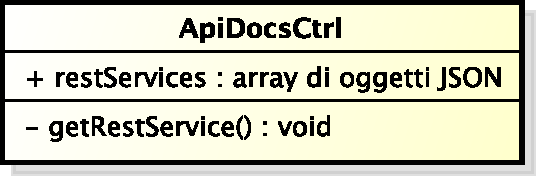
\includegraphics[scale=0.7]{./images/client/classes/controller/api_docs_ctrl.pdf}}
				\caption{Classe - client::controller::public::ApiDocsCtrl}
			\end{figure}
		\begin{itemize}
			\item \textbf{Descrizione}: la classe è il controller che serve a gestire la logica applicativa riguardante la pagina di visualizzazione dei servizi REST che il sistema offre;
			\item \textbf{Utilizzo}: viene utilizzata per gestire in maniera automatica la documentazione riguardante i servizi REST offerti dal sistema;
			\item \textbf{Relazioni con altre classi}:
				\begin{itemize}
					\item client::model::ApiDocsModel
					\item client::view::public::ApiDocs
					\item client::controller::public::PublicRoute
				\end{itemize}

			\item \textbf{Attributi associati allo \$scope}:
				\begin{itemize}
					\item \textcolor{forestgreen}{\texttt{+ restServices : array di oggetti JSON }}
						\begin{description}
							\item \textbf{Descrizione}: array di oggetti nel formato JSON che rappresentano la lista delle API pubbliche. Questa variabile viene inizializzata tramite la chiamata immediata alla funzione privata getRestService.
						\end{description}
				\end{itemize}

			\item \textbf{Metodi associati allo \$scope e privati}:
				\begin{itemize}
					\item \textcolor{forestgreen}{\texttt{- getRestService()}}
						\begin{description}
							\item \textbf{Descrizione}: metodo che preleva la lista delle API pubbliche tramite una chiamata alla classe ApiDocsModel.
						\end{description}
				\end{itemize}

			\item \textbf{Servizi AngularJS utilizzati}: N/A

		\end{itemize}
		% subparagraph bdsm_app_client_controller_public_apidocsctrl (end)


% subsubsection bdsm_app_client_controller_public (end)



\subsubsection{client::controller::user} % (fold)
\label{ssub:bdsm_app_client_controller_user}
\begin{figure}[htbp]
	\centering
	\centerline{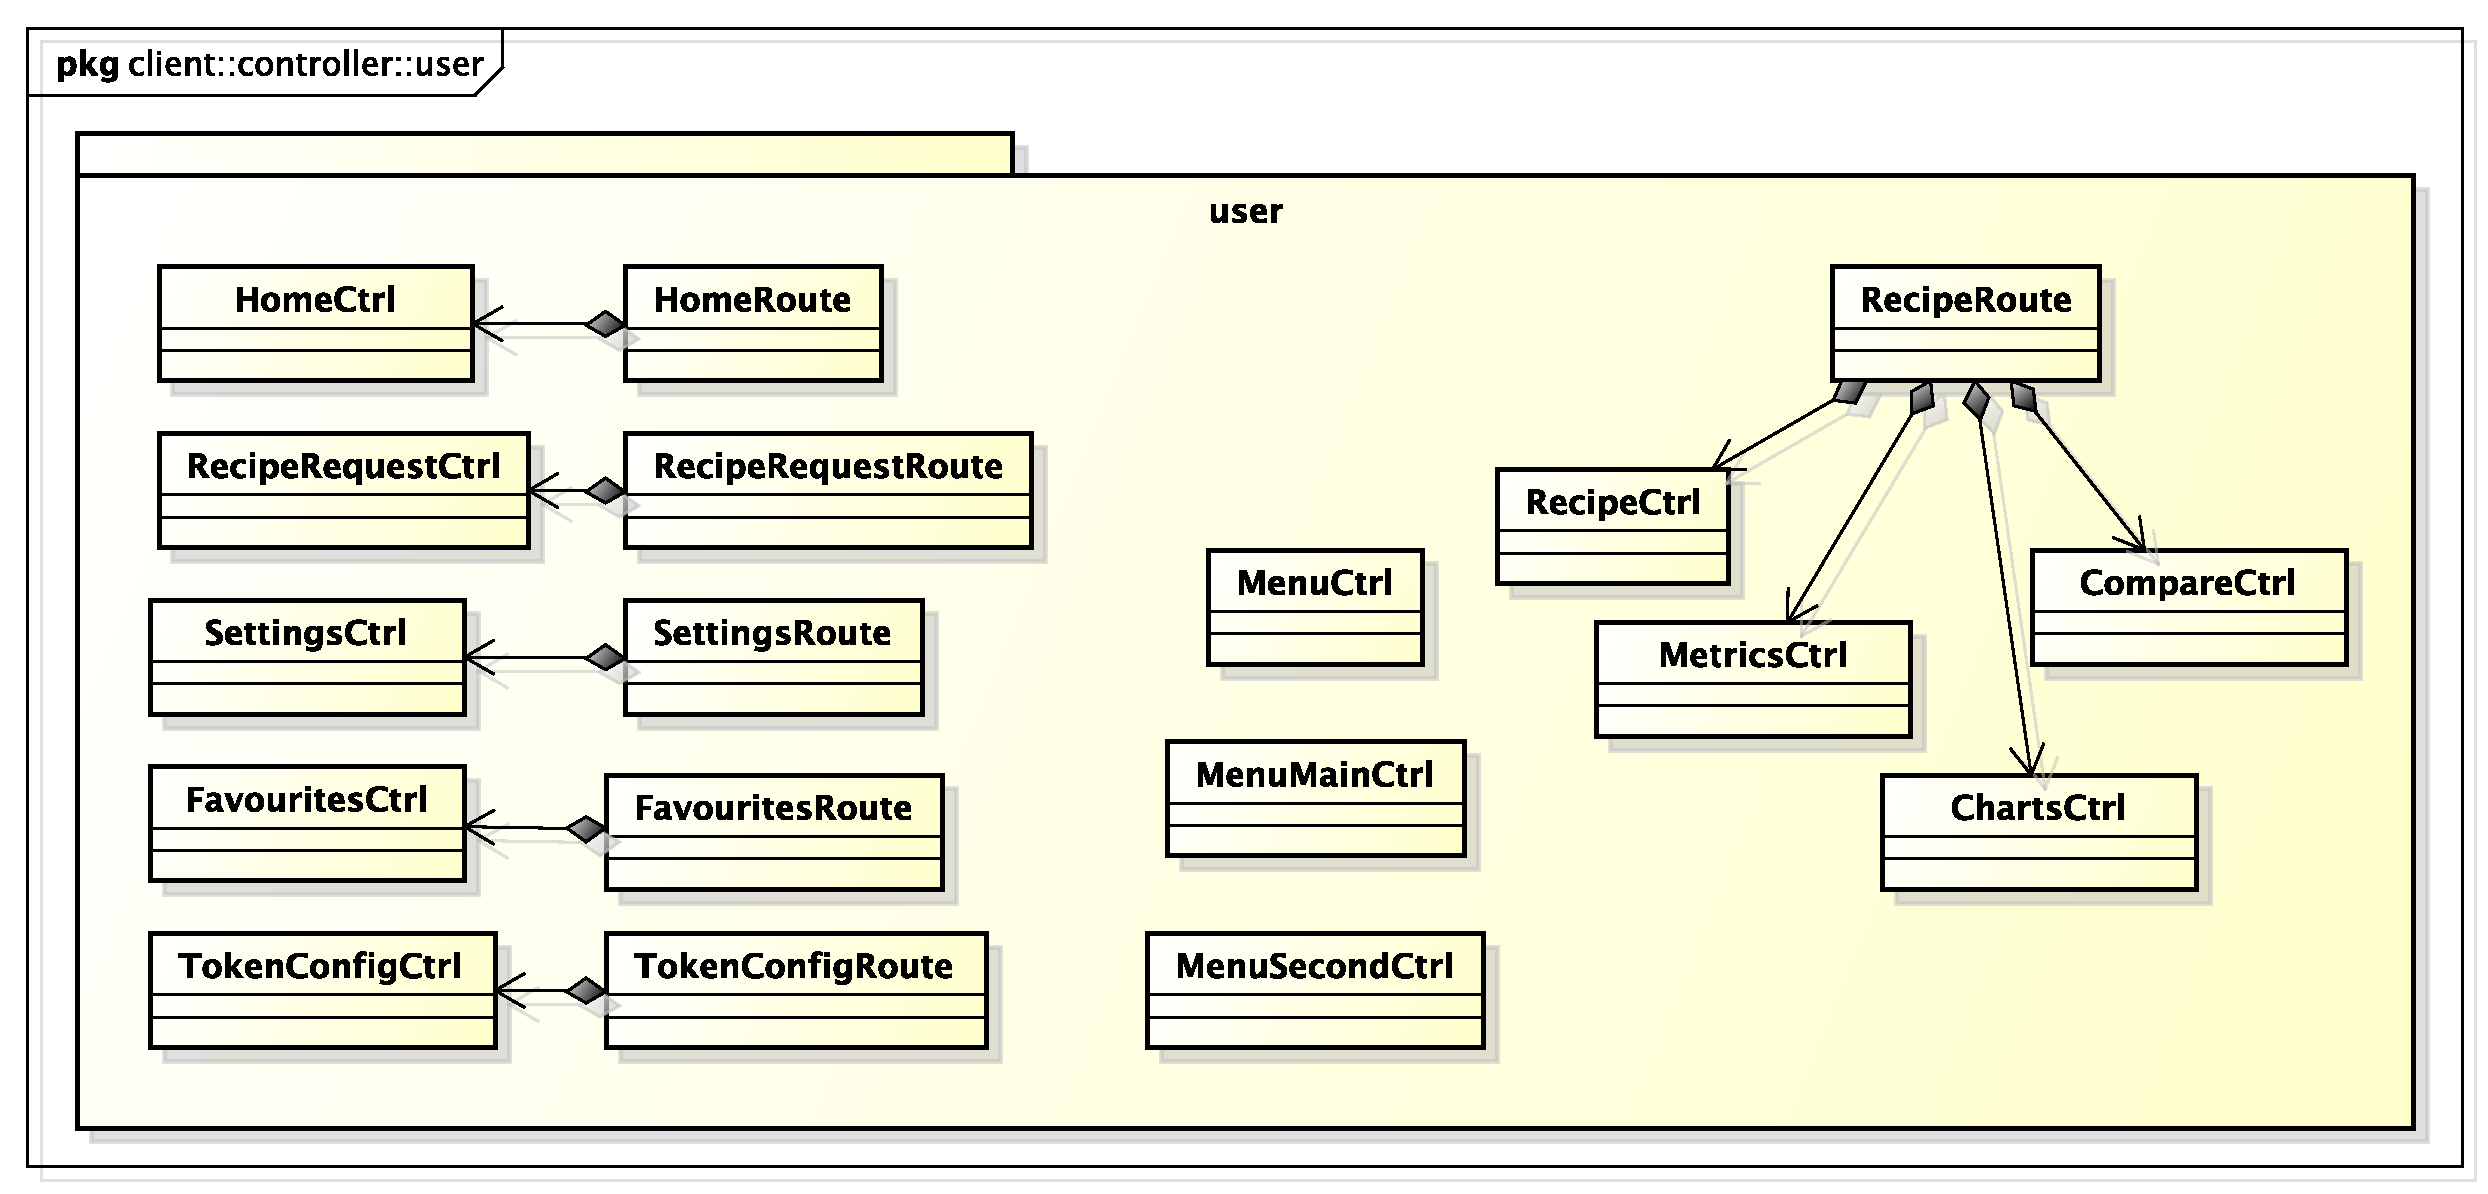
\includegraphics[scale=0.45]{./images/client/client_controller_user.pdf}}
	\caption{Package - client::controller::user}
\end{figure}

\begin{itemize}
	\item \textbf{Descrizione}: è il package che contiene le classi che controllano le decisioni di che pagine HTML mostrare all'utente autenticato e di quali operazioni poter effettuare su di esse;
	\item \textbf{Padre}: client::controller
	\item \textbf{Interazione con altri componenti}:
		\begin{itemize}
			\item client::model::user
			\item client::view::user
		\end{itemize}
\end{itemize}

	\paragraph{Classi} % (fold)
		\subparagraph{client::controller::user::MenuCtrl} % (fold)
		\label{subp:client_controller_user_menuctrl}
			\begin{itemize}
				\item \textbf{Descrizione}: la classe è il controller che serve a gestire la logica applicativa riguardante la parte in comune tra i diversi menu presenti nell'applicazione
				\item \textbf{Utilizzo}: viene utilizzata per gestire le operazioni in comune e gli stati tra i diversi menu effettivi che conterranno i vari collegamenti alle diverse pagine;
				\item \textbf{Relazioni con altre classi}:
					\begin{itemize}
						\item client::view::user::Menu
					\end{itemize}
				\item \textbf{Attributi associati allo \$scope}: N/A
				\item \textbf{Metodi associati allo \$scope e privati}: N/A
			\end{itemize}
		% subparagraph client_controller_user_menuctrl (end)

		\subparagraph{client::controller::user::MenuMainCtrl} % (fold)
		\label{subp:client_controller_user_menumainctrl}
			\begin{itemize}
				\item \textbf{Descrizione}: la classe è il controller che serve a gestire la logica applicativa riguardante il menu principale dell'applicazione;
				\item \textbf{Utilizzo}: viene utilizzata per gestire i collegamenti principali ad alcune pagine del sistema ed ad effettuare l'operazione di logout;
				\item \textbf{Classi ereditate}:
					\begin{itemize}
						\item client::controller::user::MenuCtrl. Questa ereditarietà è solo logica e non viene implementata in nessuna forma.
					\end{itemize}
				\item \textbf{Relazioni con altre classi}:
					\begin{itemize}
						\item client::view::user::MenuMain
						\item client::controller::user::LogoutCtrl
						\item client::controller::public::HomeRoute
						\item client::controller::user::SettingsRoute
					\end{itemize}
				\item \textbf{Attributi associati allo \$scope}: N/A
				\item \textbf{Metodi associati allo \$scope e privati}: N/A
				\item \textbf{Servizi AngularJS utilizzati}: N/A
			\end{itemize}
		% subparagraph client_controller_user_menumainctrl (end)

		\subparagraph{client::controller::user::MenuSecondCtrl} % (fold)
		\label{subp:client_controller_user_menusecondctrl}

			\begin{itemize}
				\item \textbf{Descrizione}: la classe è il controller che serve a gestire la logica applicativa riguardante il menu secondario dell'applicazione;
				\item \textbf{Utilizzo}: viene utilizzata per gestire i collegamenti secondari alla maggior parte delle pagine del sistema;
				\item \textbf{Classi ereditate}:
					\begin{itemize}
						\item client::controller::user::MenuCtrl. Questa ereditarietà è solo logica e non viene implementata in nessuna forma.
					\end{itemize}
				\item \textbf{Relazioni con altre classi}:
					\begin{itemize}
						\item client::view::user::MenuSecond
						\item client::controller::user::RecipeRoute
						\item client::controller::user::RecipeRequestRoute
						\item client::controller::user::FavouritesRoute
						\item client::controller::user::TokenConfigRoute
					\end{itemize}
				\item \textbf{Attributi associati allo \$scope}: N/A
				\item \textbf{Metodi associati allo \$scope e privati}: N/A
				\item \textbf{Servizi AngularJS utilizzati}: N/A
			\end{itemize}
		% subparagraph client_controller_user_menusecondctrl (end)


		\subparagraph{client::controller::user::HomeRoute} % (fold)
		\label{subp:bdsm_app_client_controller_user_homerouteconfig}
			\begin{itemize}
				\item \textbf{Descrizione}: la classe serve a gestire l'indirizzamento e l'assegnazione di uno stato al template HTML riguardante la Home page dell'utente che ha effettuato l'accesso al sistema;
				\item \textbf{Utilizzo}: viene utilizzata per reindirizzare l'utente al template HTML della pagina iniziale dell'applicativo una volta effettuato l'accesso ed assegnare al template scelto il controller opportuno per gestire i diversi compiti;
				\item \textbf{Relazioni con altre classi}:
					\begin{itemize}
						\item client::view::user::Home
						\item client::controller::user::HomeCtrl
					\end{itemize}
				\item \textbf{Attributi associati allo \$scope}: N/A
				\item \textbf{Metodi associati allo \$scope e privati}: N/A
				\item \textbf{Servizi AngularJS utilizzati}:
					\begin{itemize}
						\item \$stateProvider
					\end{itemize}
			\end{itemize}
		% subparagraph bdsm_app_client_controller_user_homerouteconfig (end)

		\subparagraph{client::controller::user::HomeCtrl} % (fold)
		\label{subp:client_controller_user_homectrl}
			\begin{itemize}
				\item \textbf{Descrizione}: la classe è il controller che serve a gestire la logica applicativa riguardante la pagina principale dell'applicazione, una volta che l'utente ha effettuato l'accesso;
				\item \textbf{Utilizzo}: viene utilizzata per gestire la pagina principale dell'applicazione. Su di essa per il momento non sono state previste particolari operazioni, ma viene lo stesso inserito un controller per scopi futuri;
				\item \textbf{Relazioni con altre classi}:
					\begin{itemize}
						\item client::view::user::Home
						\item client::controller::user::HomeRoute
					\end{itemize}

				\item \textbf{Attributi associati allo \$scope}: N/A
				\item \textbf{Metodi associati allo \$scope e privati}: N/A
				\item \textbf{Servizi AngularJS utilizzati}: N/A

			\end{itemize}
		% subparagraph client_controller_user_homectrl (end)

		\subparagraph{client::controller::user::RecipeRoute} % (fold)
		\label{subp:bdsm_app_client_controller_user_reciperouteconfig}

			\begin{itemize}
				\item \textbf{Descrizione}: la classe serve a gestire l'indirizzamento e l'assegnazione di uno stato al template HTML riguardante la pagina delle Recipe e di quelle che vengono create da essa, quali \textbf{Metrics}, \textbf{Charts} e \textbf{Compare};
				\item \textbf{Utilizzo}: viene utilizzata per reindirizzare l'utente al template HTML della pagina relativa alle Recipe presenti nel sistema ed assegnare al template scelto il controller opportuno per gestire i diversi compiti.  Da li l'utente potrà muoversi a seconda delle sue esigenze nelle pagine citate nella \emph{Descrizione};
				\item \textbf{Relazioni con altre classi}:
					\begin{itemize}
						\item client::view::user::Recipe
						\item client::view::user::Metrics
						\item client::view::user::Charts
						\item client::view::user::Compare
						\item client::controller::user::RecipeCtrl
						\item client::controller::user::MetricsCtrl
						\item client::controller::user::ChartsCtrl
						\item client::controller::user::CompareCtrl
					\end{itemize}
				\item \textbf{Attributi associati allo \$scope}: N/A
				\item \textbf{Metodi associati allo \$scope e privati}: N/A
				\item \textbf{Servizi AngularJS utilizzati}:
					\begin{itemize}
						\item \$stateProvider
					\end{itemize}
			\end{itemize}
		% subparagraph bdsm_app_client_controller_user_reciperouteconfig (end)

		\subparagraph{client::controller::user::RecipeCtrl} % (fold)
		\label{subp:client_controller_user_recipectrl}
			\begin{figure}[htbp]
				\centering
				\centerline{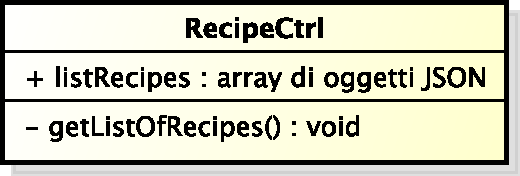
\includegraphics[scale=0.7]{./images/client/classes/controller/recipe_ctrl.pdf}}
				\caption{Classe - client::controller:user::RecipeCtrl}
			\end{figure}
			\begin{itemize}
				\item \textbf{Descrizione}: la classe è il controller che serve a gestire la logica applicativa riguardante le Recipe presenti nel sistema;
				\item \textbf{Utilizzo}: viene utilizzata per gestire la lista delle Recipe disponibili che verranno mostrate all'utente e le operazioni che esso ha a disposizione su queste. Queste operazioni saranno sotto forma di pulsanti associati a ciascuna metrica che porteranno l'utente o a visualizzare tutte le metriche inerenti alla Recipe scelta o ad effettuare un confronto tra le diverse metriche presenti;
				\item \textbf{Relazioni con altre classi}:
					\begin{itemize}
						\item client::model::services::RecipeService
						\item client::view::user::Recipe
						\item client::controller::view::RecipeRoute
					\end{itemize}

				\item \textbf{Attributi associati allo \$scope}:
					\begin{itemize}
						\item \textcolor{forestgreen}{\texttt{ + listRecipes : array di oggetti JSON}}
							\begin{description}
								\item \textbf{Descrizione}: array di oggetti nel formato JSON che rappresentano la lista delle recipe presenti nel sistema. Questa variabile viene inizializzata tramite la chiamata immediata al metodo privata getListOfRecipes. Il formato degli oggetti JSON contenuti nell'array è il seguente:
								\begin{verbatim}
									{
									    id: '42',
									    title: 'Titolo della Recipe',
									    desc: 'Descrizione della Recipe'
									}
								\end{verbatim}
							\end{description}

					\end{itemize}

				\item \textbf{Metodi associati allo \$scope e privati}:
					\begin{itemize}
						\item \textcolor{forestgreen}{\texttt{- getListOfRecipes()}}
							\begin{description}
								\item \textbf{Descrizione}: metodo che preleva la lista delle recipe tramite una chiamata al metodo \textbf{getRecipesList} della classe RecipeService.
							\end{description}

					\end{itemize}

				\item \textbf{Servizi AngularJS utilizzati}: N/A

			\end{itemize}
		% subparagraph client_controller_user_recipectrl (end)

		\subparagraph{client::controller::user::MetricsCtrl} % (fold)
		\label{subp:client_controller_user_metricsctrl}
			\begin{figure}[htbp]
				\centering
				\centerline{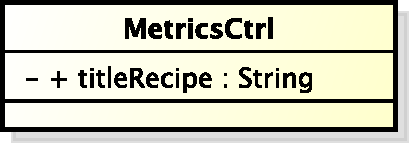
\includegraphics[scale=0.7]{./images/client/classes/controller/metrics_ctrl.pdf}}
				\caption{Classe - client::controller:user::MetricsCtrl}
			\end{figure}
			\begin{itemize}
				\item \textbf{Descrizione}: la classe è il controller che serve a gestire la logica applicativa riguardante le metriche associate ad una Recipe precisa;
				\item \textbf{Utilizzo}: viene utilizzata per gestire la lista delle metriche associate a una Recipe, fornendo dei pulsanti per ciascuna che serviranno all'utente per andare a visualizzare i grafici inerenti alla metrica selezionata;
				\item \textbf{Relazioni con altre classi}:
					\begin{itemize}
						\item client::model::services::RecipeService
						\item client::view::user::metrics
						\item client::controller::user::RecipeRoute
					\end{itemize}

				\item \textbf{Attributi associati allo \$scope}:
					\begin{itemize}
						\item \textcolor{forestgreen}{\texttt{+ titleRecipe : String}}
							\begin{description}
								\item \textbf{Descrizione}: parametro che identifica il nome della Recipe che contiene le metriche visualizzate dalla pagina. Questo parametro viene inizializzato con il valore preso in input dalla pagina delle Recipe quando si sceglie di visualizzare le metriche per una determinata di esse;
							\end{description}
						\item \textcolor{forestgreen}{\texttt{+ metricsType : array di oggetti JSON}}
							\begin{description}
								\item \textbf{Descrizione}: parametro che contiene la lista delle categorie possibile di metriche. Questo campo viene inizializzato invocando il metodo \textbf{getMetricTypes()};
							\end{description}
						\item \textcolor{forestgreen}{\texttt{+ metrics : array di oggetti JSON}}
							\begin{description}
								\item \textbf{Descrizione}: parametro che contiene la lista delle metriche di una determinata Recipe.
							\end{description}

					\end{itemize}

				\item \textbf{Metodi associati allo \$scope e privati}:
					\begin{itemize}
						\item \textcolor{forestgreen}{\texttt{- getMetricTypes() : array di oggetti JSON}}
							\begin{description}
								\item \textbf{Descrizione}: metodo che recupera il tipo di metriche presenti attraverso la chiamata \textbf{getMetricType()} al servizio \textbf{RecipeService}. L'array restituito sarà il seguente:
									\begin{verbatim}
										[
										    {
										        key: 'facebook',
										        value: 'Facebook'
										     },
										     {
										        key: 'twitter',
										        value: 'Twitter'
										      },
										      {
										         key: 'instagram',
										         value: 'Instagram'
										       }
										]
									\end{verbatim}
							\end{description}
						\item \textcolor{forestgreen}{\texttt{- getMetricsList() : void}}
							\begin{description}
								\item \textbf{Descrizione}: metodo che viene invocato quando la classe viene attivata. Questo effettua la chiamata \textbf{getMetricsList(idRecipe)} sul servizio \textbf{RecipeService} e va a riempire l'attributo \textbf{metrics} con un array di oggetti JSON del seguente formato:
								\begin{verbatim}
									    {
									        id: 'StarWars.it',
									        category: 'facebook',
									        category_type: 'page'
									     }
								\end{verbatim}
							\end{description}
					\end{itemize}

				\item \textbf{Servizi AngularJS utilizzati}: N/A

			\end{itemize}
		% subparagraph client_controller_user_metricsctrl (end)

		\subparagraph{client::controller::user::ChartsCtrl} % (fold)
		\label{subp:client_controller_user_chartsctrl}
			\begin{figure}[htbp]
				\centering
				\centerline{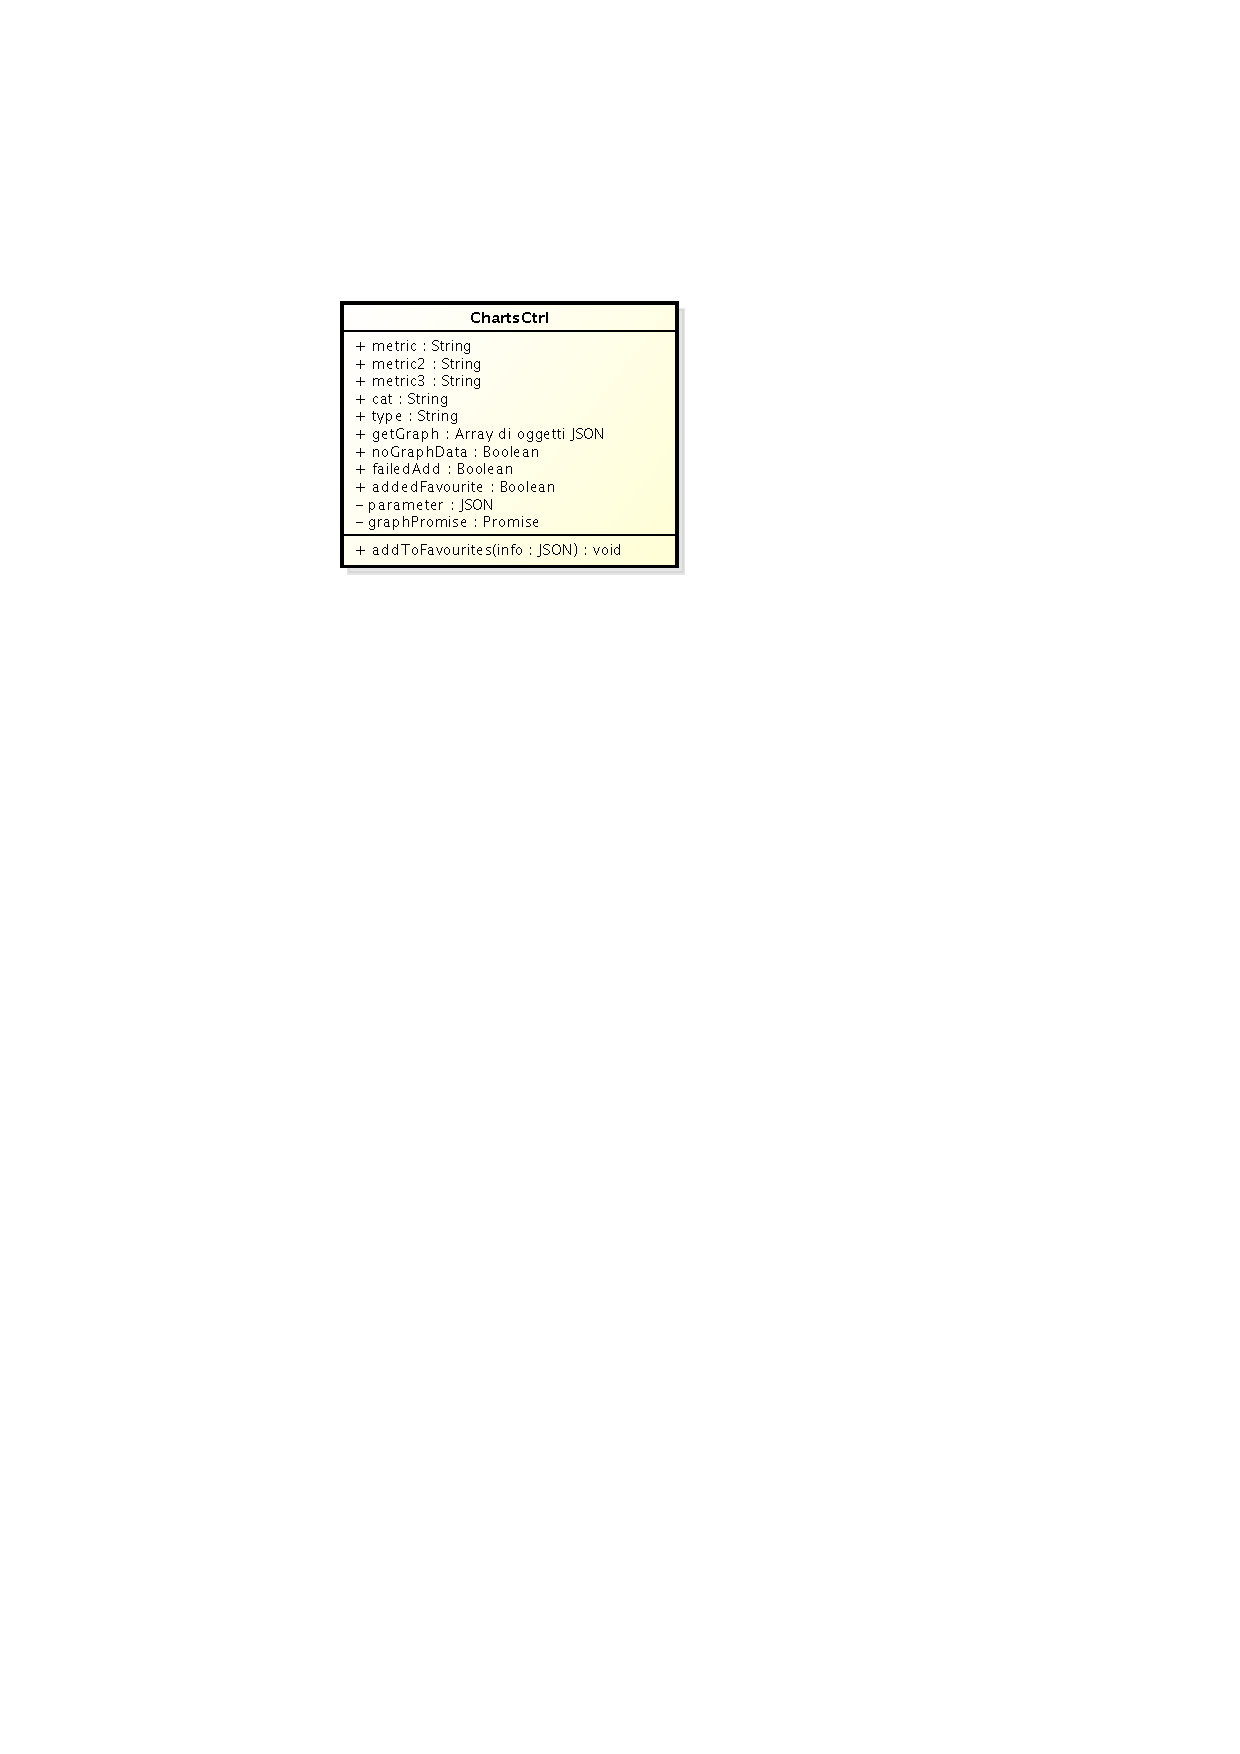
\includegraphics[scale=0.6]{./images/client/classes/controller/charts_ctrl.pdf}}
				\caption{Classe - client::controller:user::ChartsCtrl}
			\end{figure}
			\begin{itemize}
				\item \textbf{Descrizione}: la classe è il controller che serve a gestire la logica applicativa riguardante i grafici che vengono generati a partire dai dati associati ad una metrica precisa;
				\item \textbf{Utilizzo}: viene utilizzata per gestire e generare i grafici a partire dai dati della metrica selezionata. La classe richiamerà i diversi metodi presenti nel \textbf{model} che a seconda della tipologia della metrica, creeranno i grafici opportuni;
				\item \textbf{Relazioni con altre classi}:
					\begin{itemize}
						\item client::model::services::RecipeService
						\item client::view::user::Charts
						\item client::controller::user::RecipeRoute
					\end{itemize}

				\item \textbf{Attributi associati allo \$scope}:
					\begin{itemize}
						\item \textcolor{forestgreen}{\texttt{+ metric : String}}
							\begin{description}
								\item \textbf{Descrizione}: parametro che identifica il nome della metrica da cui generare i grafici. Se sono presenti altre metriche è una delle metriche da cui generare il confronto.
							\end{description}
						\item \textcolor{forestgreen}{\texttt{+ metric2 : String}}
							\begin{description}
								\item \textbf{Descrizione}: parametro opzionale, se non vuoto identifica una delle metriche con cui effettuare confronto.
							\end{description}
						\item \textcolor{forestgreen}{\texttt{+ metric3 : String}}
							\begin{description}
								\item \textbf{Descrizione}: parametro opzionale, se non vuoto identifica una delle metriche con cui effettuare confronto.
							\end{description}
						\item \textcolor{forestgreen}{\texttt{+ cat : String}}
							\begin{description}
								\item \textbf{Descrizione}: parametro che identifica la categoria della/e metrica/metriche.
							\end{description}
						\item \textcolor{forestgreen}{\texttt{+ type : String}}
							\begin{description}
								\item \textbf{Descrizione}: parametro che identifica il tipo della/e metrica/metriche.
							\end{description}
						\item \textcolor{forestgreen}{\texttt{+ graphs : Array di oggetti JSON}}
							\begin{description}
								\item \textbf{Descrizione}: contiene i grafici che devono essere visualizzati in un JSON della forma:
								\begin{verbatim}
									    {
									        desc: 'Descrizione del grafico',
									        data: codice HTML per generare il grafico
									     }
								\end{verbatim}
							\end{description}
					\end{itemize}

				\item \textbf{Metodi associati allo \$scope e privati}:
					\begin{itemize}
						\item \textcolor{forestgreen}{\texttt{- getGraphs: Array di oggetti JSON}}
							\begin{description}
								\item \textbf{Descrizione}: metodo per chiamare i metodi di RecipeService per la creazione di grafici. Ritorna un array di JSON nella forma descritta per l'attributo graphs.
							\end{description}

					\end{itemize}

				\item \textbf{Servizi AngularJS utilizzati}:
					\begin{itemize}
						\item \$stateParams
					\end{itemize}

			\end{itemize}
		% subparagraph client_controller_user_chartsctrl (end)

		\subparagraph{client::controller::user::CompareCtrl} % (fold)
		\label{subp:client_controller_user_comparectrl}
			\begin{figure}[htbp]
				\centering
				\centerline{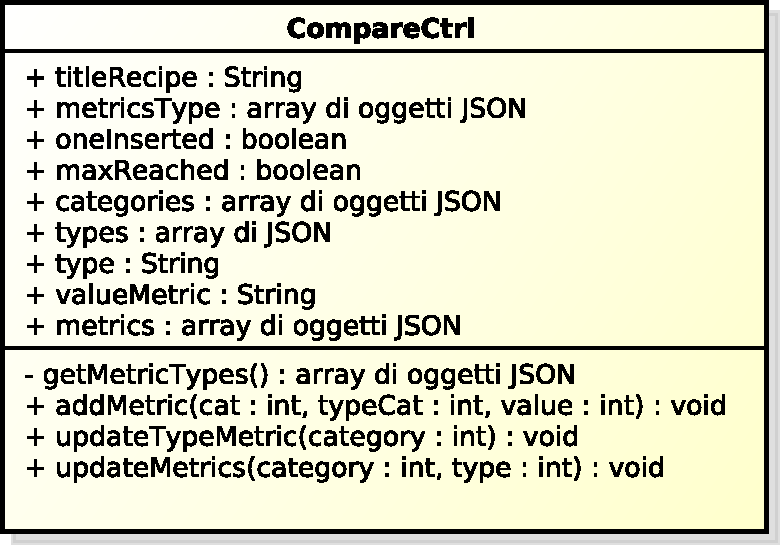
\includegraphics[scale=0.7]{./images/client/classes/controller/compare_ctrl.pdf}}
				\caption{Classe - client::controller:user::CompareCtrl}
			\end{figure}
			\begin{itemize}
				\item \textbf{Descrizione}: la classe è il controller che serve a gestire la logica applicativa riguardante la generazione di confronti tra diverse metriche di una Recipe;
				\item \textbf{Utilizzo}: viene utilizzata per gestire e generare i grafici a partire dai dati delle metriche selezionate che si vuole confrontare;
				\item \textbf{Relazioni con altre classi}:
					\begin{itemize}
						\item client::model::data::CompareModel
						\item client::view::user::Compare
						\item client::controller::RecipeRoute
					\end{itemize}

				\item \textbf{Attributi associati allo \$scope}:
					\begin{itemize}
						\item \textcolor{forestgreen}{\texttt{+ titleRecipe : String}}
							\begin{description}
								\item \textbf{Descrizione}: parametro che identifica il nome della Recipe della quale si vogliono usare le metriche per effettuare un confronto. Questo parametro viene inizializzato con il valore preso in input dalla pagina delle Recipe quando si sceglie di visualizzare le metriche per una determinata di esse;
							\end{description}
						\item \textcolor{forestgreen}{\texttt{+ metricsType : array di oggetti JSON}}
							\begin{description}
								\item \textbf{Descrizione}: parametro che contiene la lista delle categorie possibile di metriche. Questo campo viene inizializzato invocando il metodo \textbf{getMetricTypes()};
							\end{description}
						\item \textcolor{forestgreen}{\texttt{+ oneInserted : bool}}
							\begin{description}
								\item \textbf{Descrizione}: parametro che serve ad indicare quando almeno una metrica è stata aggiunta. Questo blocca degli elementi della form che non possono più essere modificati. Viene inizializzata a false e cambia il suo valore la prima volta che il metodo \textbf{addMetric(cat, typeCat, value)} viene eseguito;
							\end{description}
							\item \textcolor{forestgreen}{\texttt{+ maxReached : bool}}
								\begin{description}
									\item \textbf{Descrizione}: parametro che serve ad indicare se si è raggiunto il massimo numero di metriche possibili per un confronto. Viene inizializzato a false e può cambiare il suo valore all'interno del metodo \textbf{addMetric(cat, typeCat, value)};
								\end{description}
							\item \textcolor{forestgreen}{\texttt{+ categories : array di oggetti JSON}}
								\begin{description}
									\item \textbf{Descrizione}: attributo che contiene le categoria di metriche possibili. L'attributo viene inizializzato andando a prelevare i dati tramite il servizio \textbf{RecipeService} attraverso la chiamata al metodo \textbf{getMetricType()};
								\end{description}
							\item \textcolor{forestgreen}{\texttt{+ types : array di JSON}}
								\begin{description}
									\item \textbf{Descrizione}: attributo che contiene i tipi di categoria disponibili per una determinata categoria. L'attributo viene inizializzato quando viene effettuata la scelta di quale categoria si vuole inserire tramite la chiamata al metodo \textbf{updateTypeMetric(category)};
								\end{description}
							\item \textcolor{forestgreen}{\texttt{+ type : String}}
								\begin{description}
									\item \textbf{Descrizione}: attributo che identifica il tipo di metrica che si andrà ad inserire. Viene inizializzato con la stringa vuota;
								\end{description}
							\item \textcolor{forestgreen}{\texttt{+ valueMetric : String}}
								\begin{description}
									\item \textbf{Descrizione}: attributo che identifica il valore di una metrica che si andrà a richiedere. Viene inizializzato con la stringa vuota;
								\end{description}
							\item \textcolor{forestgreen}{\texttt{+ metrics : array di oggetti JSON}}
								\begin{description}
									\item \textbf{Descrizione}: attributo che contiene tutte le metriche aggiunte alla Recipe. Viene inizializzato con un array vuoto;
								\end{description}
					\end{itemize}

				\item \textbf{Metodi associati allo \$scope e privati}:
					\begin{itemize}

						\item \textcolor{forestgreen}{\texttt{- getMetricTypes() : array di oggetti JSON}}
							\begin{description}
								\item \textbf{Descrizione}: metodo che recupera il tipo di metriche presenti attraverso la chiamata \textbf{getMetricType()} al servizio \textbf{RecipeService}. L'array restituito sarà il seguente:
									\begin{verbatim}
										[
										    {
										        key: 'facebook',
										        value: 'Facebook'
										     },
										     {
										        key: 'twitter',
										        value: 'Twitter'
										      },
										      {
										         key: 'instagram',
										         value: 'Instagram'
										       }
										]
									\end{verbatim}
							\end{description}

							\item \textcolor{forestgreen}{\texttt{+ addMetric(cat, typeCat, value) : void}}
								\begin{description}
									\item \textbf{Descrizione}: metodo che aggiunge la metrica inserita nel form in un array che contiene tutte le metriche aggiunte e cioè \textbf{metrics}. Prima di inserirla controlla se i campi siano stati inseriti correttamente. Il formato dell'oggetto JSON inserito nell'array dovrà essere il seguente:
										\begin{verbatim}
											{
											    'id': val,
											    'category': cat,
											    'category_type': typeCat
											}
										\end{verbatim}
								\end{description}

							\item \textcolor{forestgreen}{\texttt{+ updateTypeMetric(category) : void}}
								\begin{description}
									\item \textbf{Descrizione}: metodo che aggiorna l'attributo \textbf{types} quando dal form viene scelta la categoria della metrica. Questi valori vengono presi dal servizio \textbf{RecipeService} attraverso la chiamata al metodo \textbf{getMetricTypeNode(category)};
								\end{description}

						\item \textcolor{forestgreen}{\texttt{+ updateMetrics(category, type) : void}}
							\begin{description}
								\item \textbf{Descrizione}: metodo che aggiorna i valori disponibili per una determinata selezione di categoria e tipo di categoria avvenuta nella form. Questo chiama il metodo \textbf{getMetricsList(idRecipe)} del servizio \textbf{RecipeService} e filtra i risultati ottenuti in base ai valori inseriti. Una volta filtrati gli associa all'attributo \textbf{metrics}.
							\end{description}
					\end{itemize}

				\item \textbf{Servizi AngularJS utilizzati}: N/A

			\end{itemize}
		% subparagraph client_controller_user_comparectrl (end)

		\subparagraph{client::controller::user::RecipeRequestRoute} % (fold)
		\label{subp:bdsm_app_client_controller_user_reciperequestrouteconfig}
			\begin{itemize}
				\item \textbf{Descrizione}: la classe serve a gestire l'indirizzamento e l'assegnazione di uno stato al template HTML riguardante la pagina che serve ad un utente per generare delle richieste di nuove Recipe da inserire nel sistema;
				\item \textbf{Utilizzo}: viene utilizzata per reindirizzare l'utente al template HTML della pagina che permette all'utente di fare delle richieste per delle nuove Recipe ed assegnare al template scelto il controller opportuno per gestire i diversi compiti;
				\item \textbf{Relazioni con altre classi}:
					\begin{itemize}
						\item client::view::user::RecipeRequest
						\item client::controller::user::RecipeRequestCtrl
					\end{itemize}
				\item \textbf{Attributi associati allo \$scope}: N/A
				\item \textbf{Metodi associati allo \$scope e privati}: N/A
				\item \textbf{Servizi AngularJS utilizzati}:
					\begin{itemize}
						\item \$stateProvider
					\end{itemize}
			\end{itemize}
		% subparagraph bdsm_app_client_controller_user_reciperequestrouteconfig (end)

		\subparagraph{client::controller::user::RecipeRequestCtrl} % (fold)
		\label{subp:client_controller_user_reciperequestctrl}
			\begin{figure}[htbp]
				\centering
				\centerline{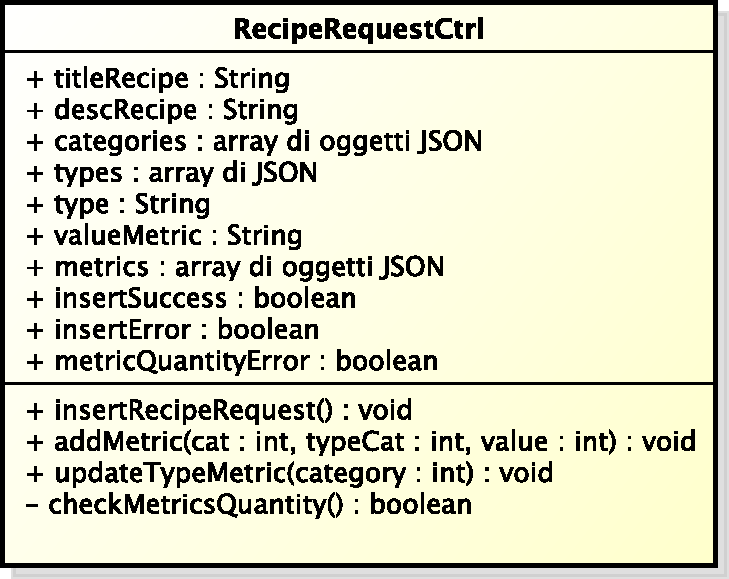
\includegraphics[scale=0.7]{./images/client/classes/controller/recipe_request_ctrl.pdf}}
				\caption{Classe - client::controller:user::RecipeRequestCtrl}
			\end{figure}
			\begin{itemize}
				\item \textbf{Descrizione}: la classe è il controller che serve a gestire la logica applicativa riguardante il form che l'utente deve compilare per effettuare una richiesta per una nuova Recipe;
				\item \textbf{Utilizzo}: viene utilizzata per gestire il form che l'utente, che desidera fare richiesta per l'inserimento di una nuova Recipe, deve compilare. La classe dovrà utilizzare il verificare in una prima istanza, la validità dei campi inseriti, anche se poi sarà il \textbf{server} ha validare effettivamente la richiesta;
				\item \textbf{Relazioni con altre classi}:
					\begin{itemize}
						\item client::model::data::RecipeRequestModel
						\item client::view::user::RecipeRequest
						\item client::controller::user::RecipeRequestRoute
					\end{itemize}

				\item \textbf{Attributi associati allo \$scope}:
					\begin{itemize}
						\item \textcolor{forestgreen}{\texttt{+ titleRecipe : String}}
							\begin{description}
								\item \textbf{Descrizione}: attributo che identifica il titolo della Recipe che si andrà a richiedere. Viene inizializzato con la stringa vuota. Questo campo è obbligatorio da inserire per poter inserire una nuova Recipe;
							\end{description}
						\item \textcolor{forestgreen}{\texttt{+ descRecipe : String}}
							\begin{description}
								\item \textbf{Descrizione}: attributo che identifica la descrizione della Recipe che si andrà a richiedere. Viene inizializzato con la stringa vuota;
							\end{description}
						\item \textcolor{forestgreen}{\texttt{+ categories : array di oggetti JSON}}
							\begin{description}
								\item \textbf{Descrizione}: attributo che contiene le categoria di metriche possibili. L'attributo viene inizializzato andando a prelevare i dati tramite il servizio \textbf{RecipeService} attraverso la chiamata al metodo \textbf{getMetricType()};
							\end{description}
						\item \textcolor{forestgreen}{\texttt{+ types : array di JSON}}
							\begin{description}
								\item \textbf{Descrizione}: attributo che contiene i tipi di categoria disponibili per una determinata categoria. L'attributo viene inizializzato quando viene effettuata la scelta di quale categoria si vuole inserire tramite la chiamata al metodo \textbf{updateTypeMetric(category)};
							\end{description}
						\item \textcolor{forestgreen}{\texttt{+ type : String}}
							\begin{description}
								\item \textbf{Descrizione}: attributo che identifica il tipo di metrica che si andrà ad inserire. Viene inizializzato con la stringa vuota;
							\end{description}
						\item \textcolor{forestgreen}{\texttt{+ valueMetric : String}}
							\begin{description}
								\item \textbf{Descrizione}: attributo che identifica il valore di una metrica che si andrà a richiedere. Viene inizializzato con la stringa vuota;
							\end{description}
						\item \textcolor{forestgreen}{\texttt{+ metrics : array di oggetti JSON}}
							\begin{description}
								\item \textbf{Descrizione}: attributo che contiene tutte le metriche aggiunte alla Recipe. Viene inizializzato con un array vuoto;
							\end{description}
						\item \textcolor{forestgreen}{\texttt{+ insertSuccess : bool}}
							\begin{description}
								\item \textbf{Descrizione}: attributo che identifica se l'inserimento della richiesta di una nuova Recipe è avvenuto con successo. Viene inizializzato a false;
							\end{description}
						\item \textcolor{forestgreen}{\texttt{+ insertError : bool}}
							\begin{description}
								\item \textbf{Descrizione}: attributo che identifica se l'inserimento della richiesta di una nuova Recipe è fallito. Viene inizializzato a false;
							\end{description}
						\item \textcolor{forestgreen}{\texttt{+ metricQuantityError : bool}}
							\begin{description}
								\item \textbf{Descrizione}: attributo che identifica se si sono inserite almeno due metriche prima di poter effettuare la richiesta di inserimento di una nuova Recipe. Viene inizializzato a false e viene modificato tramite la chiamata al metodo \textbf{checkMetricsQuantity()} nel caso la quantità fosse inferiore a quanto descritto.
							\end{description}
					\end{itemize}

				\item \textbf{Metodi associati allo \$scope e privati}:
					\begin{itemize}
						\item \textcolor{forestgreen}{\texttt{+ insertRecipeRequest() : void}}
							\begin{description}
								\item \textbf{Descrizione}: metodo che viene invocato quando si vuole inviare una nuova richiesta Recipe. Questo prima controlla se i campi obbligatori sono stati inseriti e se il numero di metriche minimo è stato aggiunto attraverso il metodo \textbf{checkMetricsQuantity()}. Se tutti i valori sono corretti allora crea un oggetto JSON con i dati prelevati dal form e chiama il metodo \textbf{createRecipe(value)} del servizio \textbf{RecipeAdminService}. Il formato dell'oggetto JSON passato dovrà essere il seguente:
									\begin{verbatim}
										{
										    'title': vm.titleRecipe,
										    'desc': vm.descRecipe,
										    'user_id': id,
										    'metrics': vm.metrics
										}
									\end{verbatim}
							\end{description}

						\item \textcolor{forestgreen}{\texttt{+ addMetric(cat, typeCat, value) : void}}
							\begin{description}
								\item \textbf{Descrizione}: metodo che aggiunge la metrica inserita nel form in un array che contiene tutte le metriche aggiunte e cioè \textbf{metrics}. Prima di inserirla controlla se i campi siano stati inseriti correttamente. Il formato dell'oggetto JSON inserito nell'array dovrà essere il seguente:
									\begin{verbatim}
										{
										    'id': val,
										    'category': cat,
										    'category_type': typeCat
										}
									\end{verbatim}
							\end{description}

						\item \textcolor{forestgreen}{\texttt{+ updateTypeMetric(category) : void}}
							\begin{description}
								\item \textbf{Descrizione}: metodo che aggiorna l'attributo \textbf{types} quando dal form viene scelta la categoria della metrica. Questi valori vengono presi dal servizio \textbf{RecipeService} attraverso la chiamata al metodo \textbf{getMetricTypeNode(category)};
							\end{description}

						\item \textcolor{forestgreen}{\texttt{- checkMetricsQuantity() : bool}}
							\begin{description}
								\item \textbf{Descrizione}: metodo che controlla che nell'array \textbf{metrics} ci siano almeno due valori e restituisce true in tal caso.
							\end{description}
					\end{itemize}

				\item \textbf{Servizi AngularJS utilizzati}: N/A


			\end{itemize}
		% subparagraph client_controller_user_reciperequestctrl (end)

		\subparagraph{client::controller::user::FavouritesRoute} % (fold)
		\label{subp:bdsm_app_client_controller_user_favouritesroute}
			\begin{itemize}
				\item \textbf{Descrizione}: la classe serve a gestire l'indirizzamento e l'assegnazione di uno stato al template HTML riguardante la pagina che serve ad un utente per guardare tutti i grafici che si è salvato tra i preferiti;
				\item \textbf{Utilizzo}: viene utilizzata per reindirizzare l'utente al template HTML della pagina che permette all'utente di visualizzare i grafici che ha tra i preferiti ed assegnare al template scelto il controller opportuno per gestire i diversi compiti;
				\item \textbf{Relazioni con altre classi}:
					\begin{itemize}
						\item client::view::user::Favourites
						\item client::controller::user::FavouritesCtrl
					\end{itemize}
				\item \textbf{Attributi associati allo \$scope}: N/A
				\item \textbf{Metodi associati allo \$scope e privati}: N/A
				\item \textbf{Servizi AngularJS utilizzati}:
					\begin{itemize}
						\item \$stateProvider
					\end{itemize}
			\end{itemize}
		% subparagraph bdsm_app_client_controller_user_favouritesroute (end)


		\subparagraph{client::controller::user::FavouritesCtrl} % (fold)
		\label{subp:client_controller_user_favouritesctrl}
			\begin{figure}[htbp]
				\centering
				\centerline{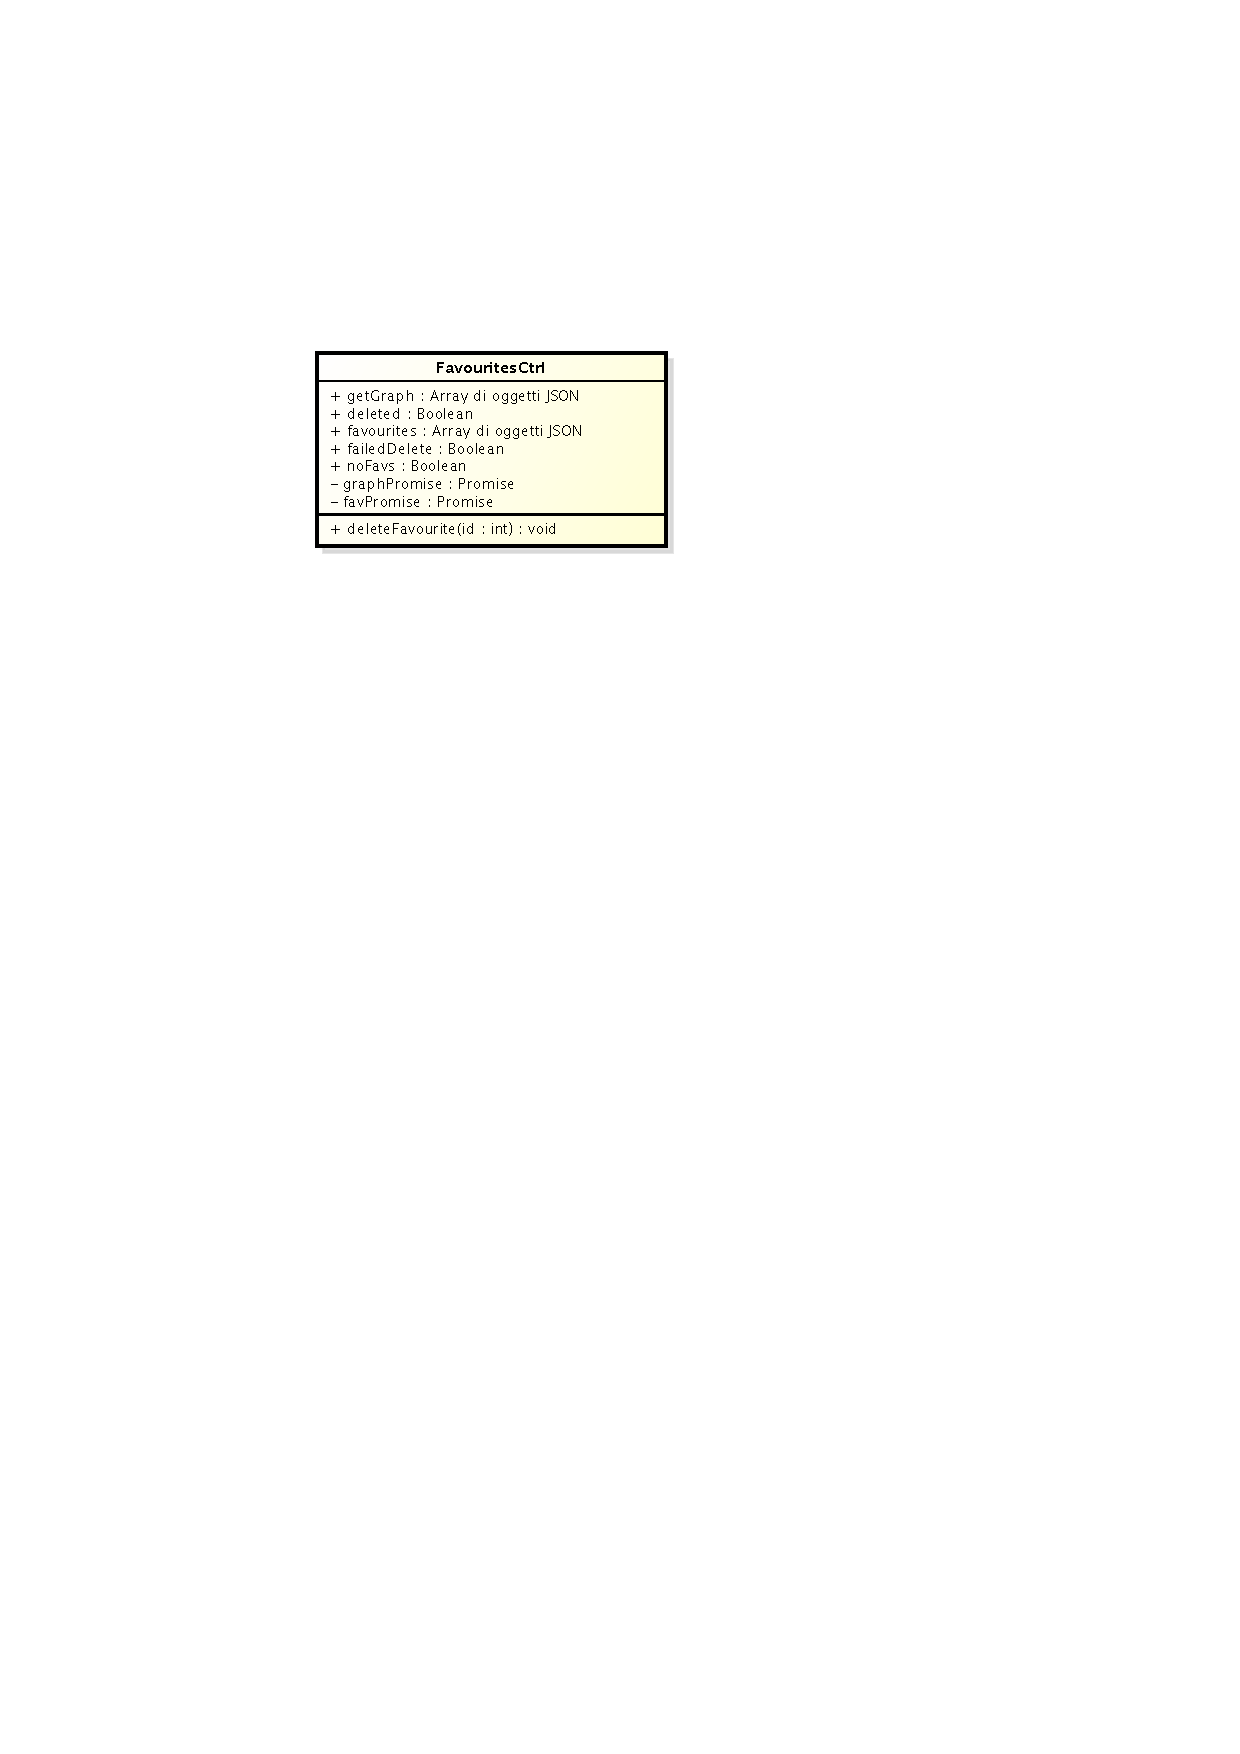
\includegraphics[scale=0.7]{./images/client/classes/controller/favourites_ctrl.pdf}}
				\caption{Classe - client::controller:user::FavouritesCtrl}
			\end{figure}
			\begin{itemize}
				\item \textbf{Descrizione}: la classe è il controller che serve a gestire la logica applicativa riguardante la pagina che mostra tutti i grafici che l'utente ha salvato tra i preferiti;
				\item \textbf{Utilizzo}: viene utilizzata per gestire tutti i grafici che l'utente ha salvato tra i preferiti;
				\item \textbf{Relazioni con altre classi}:
					\begin{itemize}
						\item client::model::services::RecipeService
						\item client::view::user::Favourites
						\item client::controller::user::FavouritesRoute
					\end{itemize}

				\item \textbf{Attributi associati allo \$scope}:
					\begin{itemize}
						\item \textcolor{forestgreen}{\texttt{+ graphs : Array di oggetti JSON}}
							\begin{description}
								\item \textbf{Descrizione}: contiene i grafici che devono essere visualizzati in un JSON della forma:
								\begin{verbatim}
									    {
									        desc: 'Descrizione del grafico',
									        data: codice HTML per generare il grafico
									     }
								\end{verbatim}
							\end{description}

					\end{itemize}

				\item \textbf{Metodi associati allo \$scope e privati}:
					\begin{itemize}
						\item \textcolor{forestgreen}{\texttt{- getFavouriteGraphs: Array di oggetti JSON}}
							\begin{description}
								\item \textbf{Descrizione}: metodo per chiamare i metodi di RecipeService per ottenere i grafici favoriti. Ritorna un array di JSON nella forma descritta per l'attributo graphs.
							\end{description}


					\end{itemize}

				\item \textbf{Servizi AngularJS utilizzati}: N/A

			\end{itemize}
		% subparagraph client_controller_user_favouritesctrl (end)

		\subparagraph{client::controller::user::TokenConfigRoute} % (fold)
		\label{subp:bdsm_app_client_controller_user_tokenconfigroute}

			\begin{itemize}
				\item \textbf{Descrizione}: la classe serve a gestire l'indirizzamento e l'assegnazione di uno stato al template HTML riguardante la pagina che serve ad un utente per generare il token che gli consente di utilizzare i servizi REST che l'applicazione offre;
				\item \textbf{Utilizzo}: viene utilizzata per reindirizzare l'utente al template HTML della pagina che permette all'utente di generare il token necessario ad utilizzare i servizi REST pubblici ed assegnare al template scelto il controller opportuno per gestire i diversi compiti;
				\item \textbf{Relazioni con altre classi}:
					\begin{itemize}
						\item client::view::user::TokenConfig
						\item client::controller::user::TokenConfigCtrl
					\end{itemize}
				\item \textbf{Attributi associati allo \$scope}: N/A
				\item \textbf{Metodi associati allo \$scope e privati}: N/A
				\item \textbf{Servizi AngularJS utilizzati}:
					\begin{itemize}
						\item \$stateProvider
					\end{itemize}
			\end{itemize}
		% subparagraph bdsm_app_client_controller_user_tokenconfigroute (end)

		\subparagraph{client::controller::user::TokenConfigCtrl} % (fold)
		\label{subp:client_controller_user_tokenconfigctrl}
			\begin{figure}[htbp]
				\centering
				\centerline{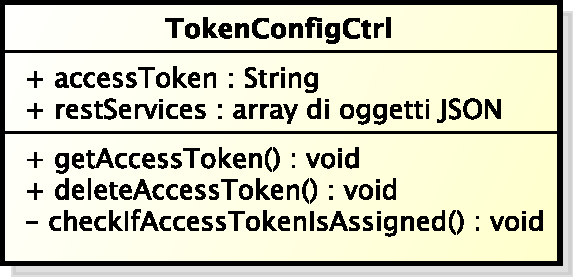
\includegraphics[scale=0.7]{./images/client/classes/controller/token_config_ctrl.pdf}}
				\caption{Classe - client::controller:user::TokenConfigCtrl}
			\end{figure}
			\begin{itemize}
				\item \textbf{Descrizione}: la classe è il controller che serve a gestire la logica applicativa riguardante la pagina che fornisce la possibilità ad un utente di ottenere un token da utilizzare per interrogare i servizi REST offerti;
				\item \textbf{Utilizzo}: viene utilizzata per gestire le operazioni che forniscono all'utente il token necessario ad interrogare i servizi REST offerti;
				\item \textbf{Relazioni con altre classi}:
					\begin{itemize}
						\item client::model::services::UserService
						\item client::view::user::TokenConfig
						\item client::controller::user::TokenConfigRoute
					\end{itemize}

				\item \textbf{Attributi associati allo \$scope}:
					\begin{itemize}
						\item \textcolor{forestgreen}{\texttt{+ accessToken : String}}
							\begin{description}
								\item \textbf{Descrizione}: attributo che identifica il token di accesso ai servizi REST utilizzabili dall'utente. Questo campo viene inizializzato con la stringa vuota se il token non è ancora stato generato, altrimenti riceve il valore corretto;
							\end{description}
						\item \textcolor{forestgreen}{\texttt{+ restServices : array di oggetti JSON}}
							\begin{description}
								\item \textbf{Descrizione}: attributo che identifica la lista dei servizi REST disponibili all'utente. Il formato degli oggetti JSON contenuti nell'array è il seguente:
								\begin{verbatim}
									{
									    type: 'GET',
									    req: '/recipes',
									    desc: 'Get the list of the available recipes'
									}
								\end{verbatim}
							\end{description}
					\end{itemize}

				\item \textbf{Metodi associati allo \$scope e privati}:
					\begin{itemize}
						\item \textcolor{forestgreen}{\texttt{+ getAccessToken() : void}}
							\begin{description}
								\item \textbf{Descrizione}: metodo che chiama il metodo \textbf{getAccessToken(idUser)} del servizio \textbf{UserService} per recuperare il token e lo assegna all'attributo \textbf{accessToken} se la chiamata è andata a buon fine;
							\end{description}
						\item \textcolor{forestgreen}{\texttt{+ deleteAccessToken() : void}}
							\begin{description}
								\item \textbf{Descrizione}: metodo che chiama il metodo \textbf{deleteAccessToken(idUser)} del servizio \textbf{UserService} per rimuovere il token e assegna all'attributo \textbf{accessToken} una stringa vuota;
							\end{description}
						\item \textcolor{forestgreen}{\texttt{- checkIfAccessTokenIsAssigned() : void}}
							\begin{description}
								\item \textbf{Descrizione}: metodo che attraverso una chiamata al metodo checkAccessToken(idUser) del servizio \textbf{UserService} salva il valore del token qualora fosse già stato generato e lo assegna all'attributo \textbf{accessToken}.
							\end{description}
					\end{itemize}

				\item \textbf{Servizi AngularJS utilizzati}: N/A

			\end{itemize}
		% subparagraph client_controller_user_tokenconfigctrl (end)

		\subparagraph{client::controller::user::SettingsRoute} % (fold)
		\label{subp:bdsm_app_client_controller_user_settingsroute}
			\begin{itemize}
				\item \textbf{Descrizione}: la classe serve a gestire l'indirizzamento e l'assegnazione di uno stato al template HTML riguardante la pagina contenente le informazioni associate ad un utente e le modifiche che può effettuare su quei dati;
				\item \textbf{Utilizzo}: viene utilizzata per reindirizzare l'utente al template HTML della pagina che permette all'utente di visualizzare le impostazione del suo profilo ed assegnare al template scelto il controller opportuno per gestire i diversi compiti;
				\item \textbf{Relazioni con altre classi}:
					\begin{itemize}
						\item client::view::user::Settings
						\item client::controller::user::SettingsCtrl
					\end{itemize}
				\item \textbf{Attributi associati allo \$scope}: N/A
				\item \textbf{Metodi associati allo \$scope e privati}: N/A
				\item \textbf{Servizi AngularJS utilizzati}:
					\begin{itemize}
						\item \$stateProvider
					\end{itemize}
			\end{itemize}
		% subparagraph bdsm_app_client_controller_user_settingsroute (end)

		\subparagraph{client::controller::user::SettingsCtrl} % (fold)
		\label{subp:client_controller_user_settingsctrl}
			\begin{figure}[htbp]
				\centering
				\centerline{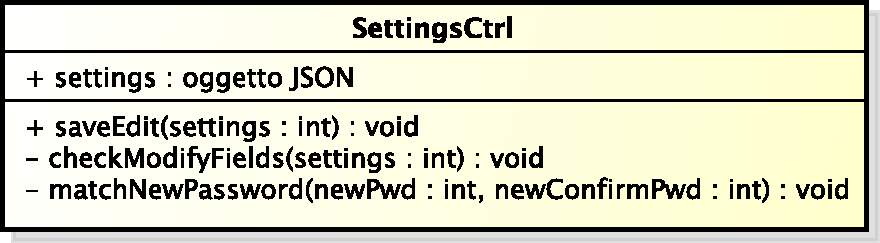
\includegraphics[scale=0.7]{./images/client/classes/controller/settings_ctrl.pdf}}
				\caption{Classe - client::controller:user::SettingsCtrl}
			\end{figure}
			\begin{itemize}
				\item \textbf{Descrizione}: la classe è il controller che serve a gestire la logica applicativa riguardante la pagina che mostra le informazioni dell'utente e la possibilità di modificarle;
				\item \textbf{Utilizzo}: viene utilizzata per gestire la visualizzazione dei dati personali associati all'utente e per le operazioni di modifica;
				\item \textbf{Relazioni con altre classi}:
					\begin{itemize}
						\item client::model::data::UserModel
						\item client::view::user::Settings
						\item client::controller::user::SettingsRoute
					\end{itemize}

				\item \textbf{Attributi associati allo \$scope}:
					\begin{itemize}
						\item \textcolor{forestgreen}{\texttt{+ settings : oggetto JSON}}
							\begin{description}
								\item \textbf{Descrizione}: oggetto nel formato JSON che contiene i valori delle impostazioni del profilo utente. I campi username e mail vengono inizializzati quando l'utente accede alla impostazioni, tramite il servizio AuthService. Il formato dell'oggetto JSON è il seguente:
								\begin{verbatim}
									{
									    username: '',
									    email: '',
									    oldPassword: '',
									    newPassword: ''
									    confirmNewPwd: ''
									}
								\end{verbatim}
							\end{description}
						\end{itemize}

				\item \textbf{Metodi associati allo \$scope e privati}:
					\begin{itemize}
						\item \textcolor{forestgreen}{\texttt{+ saveEdit(settings)}}
							\begin{description}
								\item \textbf{Descrizione}: metodo che preso in input un oggetto JSON del tipo di quello visto per l'attributo \textbf{settings} va a chiamare il servizio AuthService per salvare le modifiche effettuate. Tutto questo dopo avere controllato se la password vecchia era valida e se la password nuova combaciava con quella di conferma;
							\end{description}
						\item \textcolor{forestgreen}{\texttt{+ deleteAccount()}}
							\begin{description}
								\item \textbf{Descrizione}: metodo che cancella l'account dell'utente che ne ha richiesto la cancellazione. Questo richiama il metodo \textbf{deleteAccount(idUser)} del servizio \textbf{AuthService};
							\end{description}

						\item \textcolor{forestgreen}{\texttt{- checkModifyFields(settings)}}
							\begin{description}
								\item \textbf{Descrizione}: metodo che controlla quali campi e se sono stati modificati effettivamente e ritorna true se è stata effettuata qualche modifica e quindi ha senso chiamare il servizio per aggiornare i valori. Questo metodo viene utilizzato dentro il metodo saveEdit(settings);
							\end{description}
						\item \textcolor{forestgreen}{\texttt{- matchNewPassword(newPwd, newConfirmPwd)}}
							\begin{description}
								\item \textbf{Descrizione}: metodo che presi in input due valori, controlla se sono uguali e in tal caso restituisce true.
							\end{description}
					\end{itemize}

				\item \textbf{Servizi AngularJS utilizzati}: N/A

			\end{itemize}
		% subparagraph client_controller_user_settingsctrl (end)

		\subparagraph{client::controller::user::LogoutCtrl} % (fold) 
		\label{subp:bdsm_app_client_controller_user_logoutctrl}
			\begin{figure}[htbp]
				\centering
				\centerline{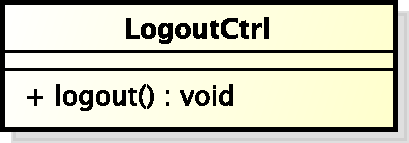
\includegraphics[scale=0.7]{./images/client/classes/controller/logout_ctrl.pdf}}
				\caption{Classe - client::controller:user::SettingsCtrl}
			\end{figure}
			\begin{itemize}
				\item \textbf{Descrizione}: la classe è il controller che serve a gestire le operazioni di logout di un utente;
				\item \textbf{Utilizzo}: viene utilizzata per distruggere la sessione attuale di un utente, attraverso la chiamata ad opportuni servizi, e il re-indirizzamento alla pagina di Login;
				\item \textbf{Relazioni con altre classi}:
					\begin{itemize}
						\item client::model::services::AuthService
						\item client::view::user::MenuMain
						\item client::controller::public::PublicRoute
					\end{itemize}
				\item \textbf{Attributi associati allo \$scope}: N/A
				\item \textbf{Metodi associati allo \$scope e privati}:
					\begin{itemize}
						\item \textcolor{forestgreen}{\texttt{+ logout()}}
							\begin{description}
								\item \textbf{Descrizione}: metodo che chiama il servizio AuthService utilizzando il metodo logout() per fare uscire l'utente dal sistema;
							\end{description}
					\end{itemize}
			\end{itemize}
		% subparagraph bdsm_app_client_controller_user_logoutctrl (end)

% subsubsection bdsm_app_client_controller_user (end)


\subsubsection{client::controller::admin} % (fold)
\label{ssub:bdsm_app_client_controller_admin}
\begin{figure}[htbp]
	\centering
	\centerline{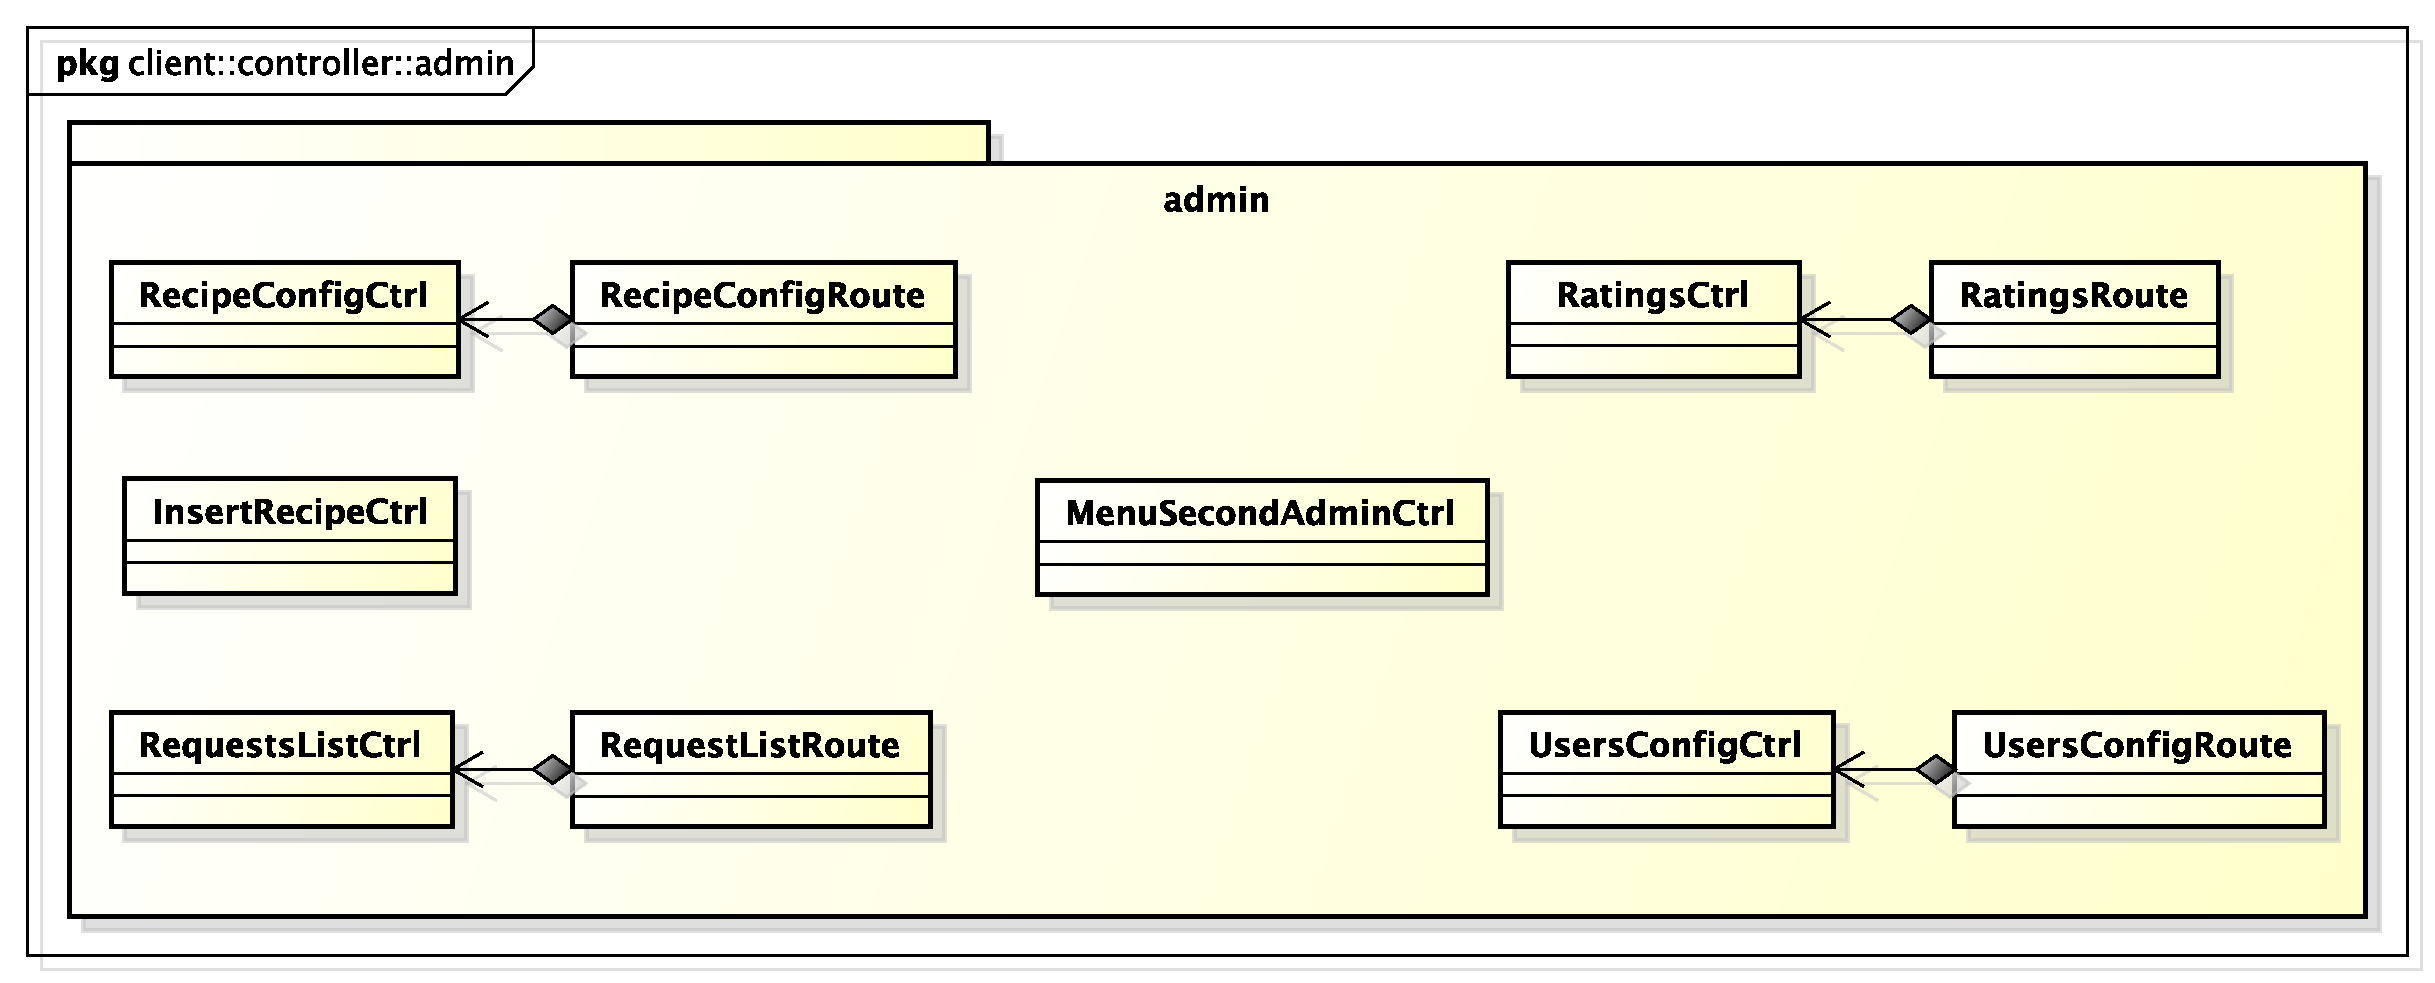
\includegraphics[scale=0.45]{./images/client/client_controller_admin.pdf}}
	\caption{Package - client::controller::admin}
\end{figure}

\begin{itemize}
	\item \textbf{Descrizione}: è il package che contiene le classi che controllano le decisioni di che pagine HTML mostrare all'amministratore e di quali operazioni poter effettuare su di esse;
	\item \textbf{Padre}: client::controller
	\item \textbf{Interazione con altri componenti}:
		\begin{itemize}
			\item client::model::admin
			\item client::view::admin
		\end{itemize}
\end{itemize}

	\paragraph{Classi} % (fold)
		\subparagraph{client::controller::admin::MenuSecondAdminCtrl} % (fold)
		\label{subp:bdsm_app_client_controller_admin_menusecondadminctrl}

			\begin{itemize}
				\item \textbf{Descrizione}: la classe è il controller che serve a gestire la logica applicativa riguardante il menu secondario dell'applicazione che ha a disposizione in più l'amministratore;
				\item \textbf{Utilizzo}: viene utilizzata per gestire i collegamenti secondari alle pagine del sistema che l'amministratore ha a disposizione per andare ad effettuare le operazioni aggiuntive a lui consentite;
				\item \textbf{Classi ereditate}:
					\begin{itemize}
						\item client::controller::user::MenuSecondCtrl. Questa ereditarietà è solo logica e non viene implementata in nessuna forma.
					\end{itemize}
				\item \textbf{Relazioni con altre classi}:
					\begin{itemize}
						\item client::view::admin::MenuSecondAdmin
						\item client::controller::admin::RecipeConfigRoute
						\item client::controller::admin::RequestListRoute
						\item client::controller::admin::RatingsRoute
						\item client::controller::admin::UserConfigRoute
					\end{itemize}
				\item \textbf{Attributi associati allo \$scope}: N/A
				\item \textbf{Metodi associati allo \$scope e privati}: N/A
			\end{itemize}
		% subparagraph bdsm_app_client_controller_admin_menusecondadminctrl (end)

		\subparagraph{client::controller::admin::RecipeConfigRoute} % (fold)
		\label{subp:bdsm_app_client_controller_admin_recipeconfigroute}

			\begin{itemize}
				\item \textbf{Descrizione}: la classe serve a gestire l'indirizzamento e l'assegnazione di uno stato al template HTML riguardante la pagina che consente di inserire una nuova Recipe nel sistema;
				\item \textbf{Utilizzo}: viene utilizzata per reindirizzare l'utente al template HTML della pagina che permette all'amministratore di andare ad inserire una nuova Recipe nel sistema ed assegnare al template scelto il controller opportuno per gestire i diversi compiti;
				\item \textbf{Relazioni con altre classi}:
					\begin{itemize}
						\item client::view::admin::RecipeConfig
						\item client::controller::admin::RecipeConfigCtrl
					\end{itemize}
				\item \textbf{Attributi associati allo \$scope}: N/A
				\item \textbf{Metodi associati allo \$scope e privati}: N/A
				\item \textbf{Servizi AngularJS utilizzati}:
					\begin{itemize}
						\item \$stateProvider
					\end{itemize}
			\end{itemize}
		% subparagraph bdsm_app_client_controller_admin_recipeconfigroute (end)

		\subparagraph{client::controller::admin::RecipeConfigCtrl} % (fold)
		\label{subp:bdsm_app_client_controller_admin_recipeconfigctrl}
			\begin{itemize}
				\item \textbf{Descrizione}: la classe è il controller che serve a gestire la logica applicativa riguardante la pagina che consente ad un amministratore di andare ad inserire una nuova Recipe;
				\item \textbf{Utilizzo}: viene utilizzata per gestire le operazioni che servono ad andare ad inserire una nuova Recipe;
				\item \textbf{Relazioni con altre classi}:
					\begin{itemize}
						\item client::model::data::RecipeInsertModel
						\item client::view::admin::RecipeConfig
						\item client::controller::admin::RecipeConfigRoute
					\end{itemize}

				\item \textbf{Attributi associati allo \$scope}: N/A
				\item \textbf{Metodi associati allo \$scope e privati}: N/A
				\item \textbf{Servizi AngularJS utilizzati}: N/A

			\end{itemize}
		% subparagraph bdsm_app_client_controller_admin_recipeconfigctrl (end)

		\subparagraph{client::controller::admin::RequestListRoute} % (fold)
		\label{subp:bdsm_app_client_controller_admin_recipelistroute}

			\begin{itemize}
				\item \textbf{Descrizione}: la classe serve a gestire l'indirizzamento e l'assegnazione di uno stato al template HTML riguardante la pagina che mostra la lista di tutte le richieste di nuove Recipe;
				\item \textbf{Utilizzo}: viene utilizzata per reindirizzare l'utente al template HTML della pagina che permette all'amministratore di visualizzare la lista di tutte le richieste di nuove Recipe proposte dagli utenti ed assegnare al template scelto il controller opportuno per gestire i diversi compiti;
				\item \textbf{Relazioni con altre classi}:
					\begin{itemize}
						\item client::view::admin::RecipeList
						\item client::controller::admin::RecipeListCtrl
					\end{itemize}
				\item \textbf{Attributi associati allo \$scope}: N/A
				\item \textbf{Metodi associati allo \$scope e privati}: N/A
				\item \textbf{Servizi AngularJS utilizzati}:
					\begin{itemize}
						\item \$stateProvider
					\end{itemize}
			\end{itemize}
		% subparagraph bdsm_app_client_controller_admin_recipelistroute (end)

		\subparagraph{client::controller::admin::RequestListCtrl} % (fold)
		\label{subp:bdsm_app_client_controller_admin_requestlistctrl}
			\begin{figure}[htbp]
				\centering
				\centerline{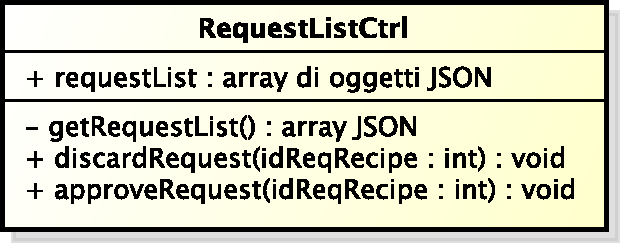
\includegraphics[scale=0.7]{./images/client/classes/controller/request_list_ctrl.pdf}}
				\caption{Classe - client::controller::admin::RequestListCtrl}
			\end{figure}
			\begin{itemize}
				\item \textbf{Descrizione}: la classe è il controller che serve a gestire la logica applicativa riguardante la pagina che consente ad un amministratore di visualizzare tutte le richieste di nuove Recipe inoltrate dagli utenti;
				\item \textbf{Utilizzo}: viene utilizzata per gestire le operazioni che servono ad andare a visualizzare la lista di tutte le richieste di nuove Recipe. Una volta scelta la richiesta da esaminare, l'amministratore potrà cliccare su un apposito pulsante per visualizzarne i dettagli;
				\item \textbf{Relazioni con altre classi}:
					\begin{itemize}
						\item client::model::services::RecipeAdminService
						\item client::view::admin::RecipeList
						\item client::controller::admin::RecipeListRoute
					\end{itemize}

				\item \textbf{Attributi associati allo \$scope}:
					\begin{itemize}
						\item \textcolor{forestgreen}{\texttt{+ requestList : array di oggetti JSON}}
							\begin{description}
								\item \textbf{Descrizione}: contiene la lista delle richieste di nuove Recipe proveniente dagli utenti non amministratori. Il formato degli oggetti JSON contenuti nell'array è il seguente:
								\begin{verbatim}
									{
									    idRequestRecipe: '42',
									    titleRecipe: 'Titolo della Recipe',
									    descRecipe: 'Descrizione della Recipe',
									    emailUser: 'info@mashup-unipd.it'
									}
								\end{verbatim}
							\end{description}

					\end{itemize}

				\item \textbf{Metodi associati allo \$scope e privati}:
					\begin{itemize}
						\item \textcolor{forestgreen}{\texttt{- getRequestList() : array JSON}}
							\begin{description}
								\item \textbf{Descrizione}: metodo che attraverso l'invocazione del metodo \textbf{getListOfRecipesRequest()} sul servizio \textbf{recipeAdminService} riceve una promessa alla chiamata effettiva per recuperare i dati dal back-end. Quando questa sarà soddisfatta, l'attributo \textbf{requestList} verrà popolato con i dati ricevuti.
							\end{description}
						\item \textcolor{forestgreen}{\texttt{+ discardRequest(idReqRecipe) : void}}
							\begin{description}
								\item \textbf{Descrizione}: metodo che attraverso l'invocazione del metodo \textbf{discardRecipeRequest(idReqRecipe)} sul servizio \textbf{recipeAdminService} riceve una promessa alla chiamata effettiva per andare a rifiutare la richiesta per quella recipe. Quando questa sarà soddisfatta, verrà visualizzato un messaggio di conferma.
							\end{description}
						\item \textcolor{forestgreen}{\texttt{+ approveRequest(idReqRecipe) : void}}
							\begin{description}
								\item \textbf{Descrizione}: metodo che attraverso l'invocazione del metodo \textbf{approveRecipeRequest(idReqRecipe)} sul servizio \textbf{recipeAdminService} riceve una promessa alla chiamata effettiva per andare ad accettare e inserire la richiesta per quella recipe. Quando questa sarà soddisfatta, verrà visualizzato un messaggio di conferma.
							\end{description}
					\end{itemize}

				\item \textbf{Servizi AngularJS utilizzati}: N/A

			\end{itemize}
		% subparagraph bdsm_app_client_controller_admin_requestlistctrl (end)

		\subparagraph{client::controller::admin::InsertRecipeCtrl} % (fold)
		\label{subp:bdsm_app_client_controller_admin_insertctrl}
			\begin{figure}[htbp]
				\centering
				\centerline{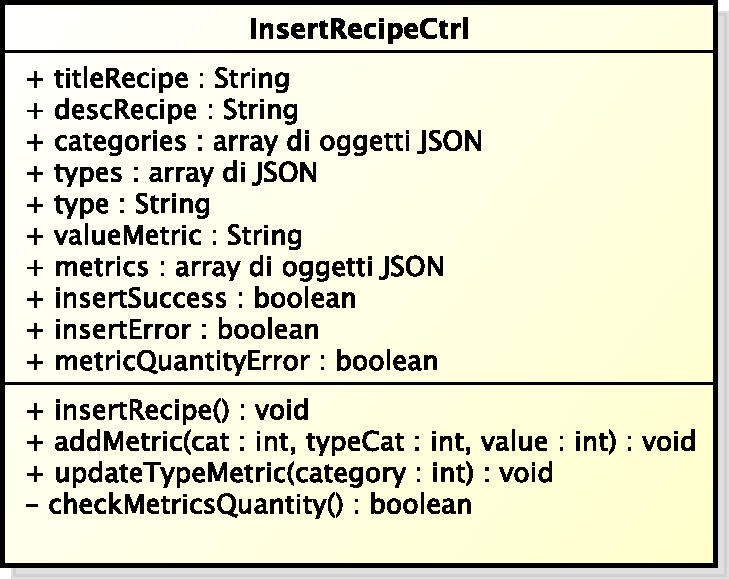
\includegraphics[scale=0.7]{./images/client/classes/controller/insert_recipe_ctrl.pdf}}
				\caption{Classe - client::controller::admin::InsertRecipeCtrl}
			\end{figure}
			\begin{itemize}
				\item \textbf{Descrizione}: la classe è il controller che serve a gestire la logica applicativa riguardante il form contenente i campi necessari all'inserimento di una nuova Recipe;
				\item \textbf{Utilizzo}: viene utilizzata per gestire il form che serve per inserire una nuova Recipe nel sistema. Può essere utilizzato sia per il form di un inserimento ex novo sia per gestire i dettagli delle richieste di nuove Recipe;
				\item \textbf{Relazioni con altre classi}:
					\begin{itemize}
						\item client::model::data::RecipeInsertModel
						\item client::view::admin::Insert
						\item client::controller::admin::RecipeConfigRoute
					\end{itemize}

				\item \textbf{Attributi associati allo \$scope}:
					\begin{itemize}
						\item \textcolor{forestgreen}{\texttt{+ titleRecipe : String}}
							\begin{description}
								\item \textbf{Descrizione}: attributo che identifica il titolo della Recipe che si andrà ad inserire. Viene inizializzato con la stringa vuota. Questo campo è obbligatorio da inserire per poter inserire una nuova Recipe;
							\end{description}
						\item \textcolor{forestgreen}{\texttt{+ descRecipe : String}}
							\begin{description}
								\item \textbf{Descrizione}: attributo che identifica la descrizione della Recipe che si andrà ad inserire. Viene inizializzato con la stringa vuota;
							\end{description}
						\item \textcolor{forestgreen}{\texttt{+ categories : array di oggetti JSON}}
							\begin{description}
								\item \textbf{Descrizione}: attributo che contiene le categoria di metriche possibili. L'attributo viene inizializzato andando a prelevare i dati tramite il servizio \textbf{RecipeService} attraverso la chiamata al metodo \textbf{getMetricType()};
							\end{description}
						\item \textcolor{forestgreen}{\texttt{+ types : array di JSON}}
							\begin{description}
								\item \textbf{Descrizione}: attributo che contiene i tipi di categoria disponibili per una determinata categoria. L'attributo viene inizializzato quando viene effettuata la scelta di quale categoria si vuole inserire tramite la chiamata al metodo \textbf{updateTypeMetric(category)};
							\end{description}
						\item \textcolor{forestgreen}{\texttt{+ type : String}}
							\begin{description}
								\item \textbf{Descrizione}: attributo che identifica il tipo di metrica che si andrà ad inserire. Viene inizializzato con la stringa vuota;
							\end{description}
						\item \textcolor{forestgreen}{\texttt{+ valueMetric : String}}
							\begin{description}
								\item \textbf{Descrizione}: attributo che identifica il valore di una metrica che si andrà ad inserire. Viene inizializzato con la stringa vuota;
							\end{description}
						\item \textcolor{forestgreen}{\texttt{+ metrics : array di oggetti JSON}}
							\begin{description}
								\item \textbf{Descrizione}: attributo che contiene tutte le metriche aggiunte alla Recipe. Viene inizializzato con un array vuoto;
							\end{description}
						\item \textcolor{forestgreen}{\texttt{+ insertSuccess : bool}}
							\begin{description}
								\item \textbf{Descrizione}: attributo che identifica se l'inserimento della nuova Recipe è avvenuto con successo. Viene inizializzato a false;
							\end{description}
						\item \textcolor{forestgreen}{\texttt{+ insertError : bool}}
							\begin{description}
								\item \textbf{Descrizione}: attributo che identifica se l'inserimento della nuova Recipe è fallito. Viene inizializzato a false;
							\end{description}
						\item \textcolor{forestgreen}{\texttt{+ metricQuantityError : bool}}
							\begin{description}
								\item \textbf{Descrizione}: attributo che identifica se si sono inserite almeno due metriche prima di poter effettuare l'inserimento di una nuova Recipe. Viene inizializzato a false e viene modificato tramite la chiamata al metodo \textbf{checkMetricsQuantity()} nel caso la quantità fosse inferiore a quanto descritto.
							\end{description}
					\end{itemize}

				\item \textbf{Metodi associati allo \$scope e privati}:
					\begin{itemize}
						\item \textcolor{forestgreen}{\texttt{+ insertRecipe() : void}}
							\begin{description}
								\item \textbf{Descrizione}: metodo che viene invocato quando si vuole inserire una nuova Recipe. Questo prima controlla se i campi obbligatori sono stati inseriti e se il numero di metriche minimo è stato aggiunto attraverso il metodo \textbf{checkMetricsQuantity()}. Se tutti i valori sono corretti allora crea un oggetto JSON con i dati prelevati dal form e chiama il metodo \textbf{createRecipe(value)} del servizio \textbf{RecipeAdminService}. Il formato dell'oggetto JSON passato dovrà essere il seguente:
									\begin{verbatim}
										{
										    'title': vm.titleRecipe,
										    'desc': vm.descRecipe,
										    'admin_id': id,
										    'metrics': vm.metrics
										}
									\end{verbatim}
							\end{description}

						\item \textcolor{forestgreen}{\texttt{+ addMetric(cat, typeCat, value) : void}}
							\begin{description}
								\item \textbf{Descrizione}: metodo che aggiunge la metrica inserita nel form in un array che contiene tutte le metriche aggiunte e cioè \textbf{metrics}. Prima di inserirla controlla se i campi siano stati inseriti correttamente. Il formato dell'oggetto JSON inserito nell'array dovrà essere il seguente:
									\begin{verbatim}
										{
										    'id': val,
										    'category': cat,
										    'category_type': typeCat
										}
									\end{verbatim}
							\end{description}

						\item \textcolor{forestgreen}{\texttt{+ updateTypeMetric(category) : void}}
							\begin{description}
								\item \textbf{Descrizione}: metodo che aggiorna l'attributo \textbf{types} quando dal form viene scelta la categoria della metrica. Questi valori vengono presi dal servizio \textbf{RecipeService} attraverso la chiamata al metodo \textbf{getMetricTypeNode(category)};
							\end{description}

						\item \textcolor{forestgreen}{\texttt{- checkMetricsQuantity() : bool}}
							\begin{description}
								\item \textbf{Descrizione}: metodo che controlla che nell'array \textbf{metrics} ci siano almeno due valori e restituisce true in tal caso.
							\end{description}
					\end{itemize}

				\item \textbf{Servizi AngularJS utilizzati}: N/A

			\end{itemize}
		% subparagraph bdsm_app_client_controller_admin_insertctrl (end)

		\subparagraph{client::controller::admin::RatingsRoute} % (fold)
		\label{subp:bdsm_app_client_controller_admin_ratingsroute}
			\begin{itemize}
				\item \textbf{Descrizione}: la classe serve a gestire l'indirizzamento e l'assegnazione di uno stato al template HTML riguardante la pagina che mostra la lista di tutte le Recipe votate con la media del valore assegnato dagli utenti;
				\item \textbf{Utilizzo}: viene utilizzata per reindirizzare l'utente al template HTML della pagina che permette all'amministratore di visualizzare la lista di tutte le Recipe votate, in ordine dalla più votata, ed assegnare al template scelto il controller opportuno per gestire i diversi compiti;
				\item \textbf{Relazioni con altre classi}:
					\begin{itemize}
						\item client::view::admin::Ratings
						\item client::controller::admin::RatingsCtrl
					\end{itemize}
				\item \textbf{Attributi associati allo \$scope}: N/A
				\item \textbf{Metodi associati allo \$scope e privati}: N/A
				\item \textbf{Servizi AngularJS utilizzati}:
					\begin{itemize}
						\item \$stateProvider
					\end{itemize}
			\end{itemize}
		% subparagraph bdsm_app_client_controller_admin_ratingsroute (end)

		\subparagraph{client::controller::admin::RatingsCtrl} % (fold)
		\label{subp:bdsm_app_client_controller_admin_ratingsctrl}
			\begin{figure}[htbp]
				\centering
				\centerline{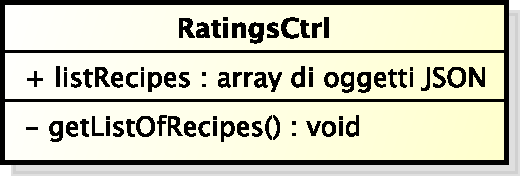
\includegraphics[scale=0.7]{./images/client/classes/controller/ratings_ctrl.pdf}}
				\caption{Classe - client::controller::admin::RatingsCtrl}
			\end{figure}
			\begin{itemize}
				\item \textbf{Descrizione}: la classe è il controller che serve a gestire la logica applicativa riguardante la pagina che consente ad un amministratore di visualizzare tutte le Recipe che sono state votate dagli utenti;
				\item \textbf{Utilizzo}: viene utilizzata per gestire le operazioni che servono ad andare a visualizzare la lista di tutte le Recipe che sono state votate dagli utenti, ordinandole dalla più votata alla meno;
				\item \textbf{Relazioni con altre classi}:
					\begin{itemize}
						\item client::model::services::RecipeAdminService
						\item client::view::admin::Ratings
						\item client::controller::admin::RatingsRoute
					\end{itemize}

				\item \textbf{Attributi associati allo \$scope}:
					\begin{itemize}
						\item \textcolor{forestgreen}{\texttt{+ listRecipes : array di oggetti JSON}}
							\begin{description}
								\item \textbf{Descrizione}: attributo che contiene la lista di tutte le Recipe aventi una valutazione. Il formato degli oggetti JSON contenuti nell'array è il seguente:
								\begin{verbatim}
									{
									    id: '42',
									    title: 'Titolo della Recipe',
									    desc: 'Descrizione della Recipe',
									    ratings: '3.44'
									}
								\end{verbatim}
							\end{description}

					\end{itemize}

				\item \textbf{Metodi associati allo \$scope e privati}:
					\begin{itemize}
						\item \textcolor{forestgreen}{\texttt{- getListOfRecipes() : void}}
							\begin{description}
								\item \textbf{Descrizione}: metodo che recupera la lista della recipe, aventi una valutazione, attraverso la chiamata del metodo \textbf{getRecipesListAll()} del servizio \textbf{recipeAdminService}. Quando i dati sono disponibili, riempe l'array \textbf{listRecipes}. L'invocazione del metodo avviene subito nel momento in cui un utente accede alla pagina \textbf{Ratings}.
							\end{description}

					\end{itemize}

				\item \textbf{Servizi AngularJS utilizzati}: N/A

			\end{itemize}
		% subparagraph bdsm_app_client_controller_admin_ratingsctrl (end)

		\subparagraph{client::controller::admin::UserConfigRoute} % (fold)
		\label{subp:bdsm_app_client_controller_admin_userconfigroute}

			\begin{itemize}
				\item \textbf{Descrizione}: la classe serve a gestire l'indirizzamento e l'assegnazione di uno stato al template HTML riguardante la pagina che mostra la lista degli utenti registrati al sistema;
				\item \textbf{Utilizzo}: viene utilizzata per reindirizzare l'utente al template HTML della pagina che permette all'amministratore di visualizzare la lista degli utenti registrati al sistema ed assegnare al template scelto il controller opportuno per gestire i diversi compiti;
				\item \textbf{Relazioni con altre classi}:
					\begin{itemize}
						\item client::view::admin::UserConfig
						\item client::controller::admin::UserConfigCtrl
					\end{itemize}
				\item \textbf{Attributi associati allo \$scope}: N/A
				\item \textbf{Metodi associati allo \$scope e privati}: N/A
				\item \textbf{Servizi AngularJS utilizzati}:
					\begin{itemize}
						\item \$stateProvider
					\end{itemize}
			\end{itemize}
		% subparagraph bdsm_app_client_controller_admin_userconfigroute (end)

		\subparagraph{client::controller::admin::UserConfigCtrl} % (fold)
		\label{subp:bdsm_app_client_controller_admin_userconfigctrl}
			\begin{figure}[htbp]
				\centering
				\centerline{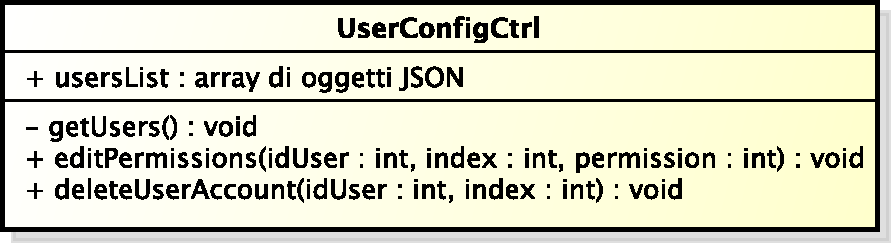
\includegraphics[scale=0.7]{./images/client/classes/controller/user_config_ctrl.pdf}}
				\caption{Classe - client::controller::admin::UserConfigCtrl}
			\end{figure}
			\begin{itemize}
				\item \textbf{Descrizione}: la classe è il controller che serve a gestire la logica applicativa riguardante la pagina che consente ad un amministratore di visualizzare la lista degli utenti registrati al sistema;
				\item \textbf{Utilizzo}: viene utilizzata per gestire le operazioni che servono ad andare a visualizzare la lista degli utenti registrati al sistema, potendo su di essi, andare a modificarne i permessi o a cancellare l'account;
				\item \textbf{Relazioni con altre classi}:
					\begin{itemize}
						\item client::model::services::UserAdminService
						\item client::view::admin::UserConfig
						\item client::controller::admin::UserConfigRoute
					\end{itemize}

				\item \textbf{Attributi associati allo \$scope}:
					\begin{itemize}
						\item \textcolor{forestgreen}{\texttt{+ usersList} : array di oggetti JSON}
							\begin{description}
								\item \textbf{Descrizione}: attributo che contiene la lista di tutti gli utenti registrati nel sistema. Il formato degli oggetti JSON contenuti nell'array è il seguente:
								\begin{verbatim}
									{
									    access_token: '3253224346356',
									    username: 'MashUp',
									    email: 'info@mashup-unipd.it',
									    permission: 'user'
									}
								\end{verbatim}
							\end{description}

					\end{itemize}

				\item \textbf{Metodi associati allo \$scope e privati}:
					\begin{itemize}
						\item \textcolor{forestgreen}{\texttt{- getUsers() : void}}
							\begin{description}
								\item \textbf{Descrizione}: metodo che recupera la lista degli utenti attraverso la chiamata del metodo \textbf{getListOfUsers} del servizio \textbf{userAdminService}. Quando i dati sono disponibili, riempe l'array \textbf{usersList}. L'invocazione del metodo avviene subito nel momento in cui un utente accede alla pagina \textbf{UsersConfig};
							\end{description}
						\item \textcolor{forestgreen}{\texttt{+ editPermissions(idUser, index, permission) : void}}
							\begin{description}
								\item \textbf{Descrizione}: metodo che modifica il tipo dell'utente, attraverso la chiamata del metodo \textbf{editUserPermissions(idUser, permission)} del servizio \textbf{userAdminService}. Quando la modifica è stata effettuata viene visualizzato un messaggio di successo e viene anche modificato il valore relativo presente nell'array \textbf{usersList} in modo da rispecchiare visivamente la diversa situazione;
							\end{description}
						\item \textcolor{forestgreen}{\texttt{+ deleteUserAccount(idUser, index) : void}}
							\begin{description}
								\item \textbf{Descrizione}: metodo che cancella l'utente, attraverso la chiamata del metodo \textbf{deleteUserAccount(idUser)} del servizio \textbf{userAdminService}. Quando la cancellazione è stata effettuata viene visualizzato un messaggio di successo e viene anche rimosso il valore relativo presente nell'array \textbf{usersList} in modo da rispecchiare visivamente la diversa situazione.
							\end{description}
					\end{itemize}

				\item \textbf{Servizi AngularJS utilizzati}: N/A
			\end{itemize}
		% subparagraph bdsm_app_client_controller_admin_userconfigctrl (end)


% subsubsection bdsm_app_client_controller_admin (end)
